% Options for packages loaded elsewhere
\PassOptionsToPackage{unicode}{hyperref}
\PassOptionsToPackage{hyphens}{url}
%
\documentclass[
]{article}
\usepackage{amsmath,amssymb}
\usepackage{iftex}
\ifPDFTeX
  \usepackage[T1]{fontenc}
  \usepackage[utf8]{inputenc}
  \usepackage{textcomp} % provide euro and other symbols
\else % if luatex or xetex
  \usepackage{unicode-math} % this also loads fontspec
  \defaultfontfeatures{Scale=MatchLowercase}
  \defaultfontfeatures[\rmfamily]{Ligatures=TeX,Scale=1}
\fi
\usepackage{lmodern}
\ifPDFTeX\else
  % xetex/luatex font selection
\fi
% Use upquote if available, for straight quotes in verbatim environments
\IfFileExists{upquote.sty}{\usepackage{upquote}}{}
\IfFileExists{microtype.sty}{% use microtype if available
  \usepackage[]{microtype}
  \UseMicrotypeSet[protrusion]{basicmath} % disable protrusion for tt fonts
}{}
\makeatletter
\@ifundefined{KOMAClassName}{% if non-KOMA class
  \IfFileExists{parskip.sty}{%
    \usepackage{parskip}
  }{% else
    \setlength{\parindent}{0pt}
    \setlength{\parskip}{6pt plus 2pt minus 1pt}}
}{% if KOMA class
  \KOMAoptions{parskip=half}}
\makeatother
\usepackage{xcolor}
\usepackage[margin=1in]{geometry}
\usepackage{color}
\usepackage{fancyvrb}
\newcommand{\VerbBar}{|}
\newcommand{\VERB}{\Verb[commandchars=\\\{\}]}
\DefineVerbatimEnvironment{Highlighting}{Verbatim}{commandchars=\\\{\}}
% Add ',fontsize=\small' for more characters per line
\usepackage{framed}
\definecolor{shadecolor}{RGB}{248,248,248}
\newenvironment{Shaded}{\begin{snugshade}}{\end{snugshade}}
\newcommand{\AlertTok}[1]{\textcolor[rgb]{0.94,0.16,0.16}{#1}}
\newcommand{\AnnotationTok}[1]{\textcolor[rgb]{0.56,0.35,0.01}{\textbf{\textit{#1}}}}
\newcommand{\AttributeTok}[1]{\textcolor[rgb]{0.13,0.29,0.53}{#1}}
\newcommand{\BaseNTok}[1]{\textcolor[rgb]{0.00,0.00,0.81}{#1}}
\newcommand{\BuiltInTok}[1]{#1}
\newcommand{\CharTok}[1]{\textcolor[rgb]{0.31,0.60,0.02}{#1}}
\newcommand{\CommentTok}[1]{\textcolor[rgb]{0.56,0.35,0.01}{\textit{#1}}}
\newcommand{\CommentVarTok}[1]{\textcolor[rgb]{0.56,0.35,0.01}{\textbf{\textit{#1}}}}
\newcommand{\ConstantTok}[1]{\textcolor[rgb]{0.56,0.35,0.01}{#1}}
\newcommand{\ControlFlowTok}[1]{\textcolor[rgb]{0.13,0.29,0.53}{\textbf{#1}}}
\newcommand{\DataTypeTok}[1]{\textcolor[rgb]{0.13,0.29,0.53}{#1}}
\newcommand{\DecValTok}[1]{\textcolor[rgb]{0.00,0.00,0.81}{#1}}
\newcommand{\DocumentationTok}[1]{\textcolor[rgb]{0.56,0.35,0.01}{\textbf{\textit{#1}}}}
\newcommand{\ErrorTok}[1]{\textcolor[rgb]{0.64,0.00,0.00}{\textbf{#1}}}
\newcommand{\ExtensionTok}[1]{#1}
\newcommand{\FloatTok}[1]{\textcolor[rgb]{0.00,0.00,0.81}{#1}}
\newcommand{\FunctionTok}[1]{\textcolor[rgb]{0.13,0.29,0.53}{\textbf{#1}}}
\newcommand{\ImportTok}[1]{#1}
\newcommand{\InformationTok}[1]{\textcolor[rgb]{0.56,0.35,0.01}{\textbf{\textit{#1}}}}
\newcommand{\KeywordTok}[1]{\textcolor[rgb]{0.13,0.29,0.53}{\textbf{#1}}}
\newcommand{\NormalTok}[1]{#1}
\newcommand{\OperatorTok}[1]{\textcolor[rgb]{0.81,0.36,0.00}{\textbf{#1}}}
\newcommand{\OtherTok}[1]{\textcolor[rgb]{0.56,0.35,0.01}{#1}}
\newcommand{\PreprocessorTok}[1]{\textcolor[rgb]{0.56,0.35,0.01}{\textit{#1}}}
\newcommand{\RegionMarkerTok}[1]{#1}
\newcommand{\SpecialCharTok}[1]{\textcolor[rgb]{0.81,0.36,0.00}{\textbf{#1}}}
\newcommand{\SpecialStringTok}[1]{\textcolor[rgb]{0.31,0.60,0.02}{#1}}
\newcommand{\StringTok}[1]{\textcolor[rgb]{0.31,0.60,0.02}{#1}}
\newcommand{\VariableTok}[1]{\textcolor[rgb]{0.00,0.00,0.00}{#1}}
\newcommand{\VerbatimStringTok}[1]{\textcolor[rgb]{0.31,0.60,0.02}{#1}}
\newcommand{\WarningTok}[1]{\textcolor[rgb]{0.56,0.35,0.01}{\textbf{\textit{#1}}}}
\usepackage{graphicx}
\makeatletter
\def\maxwidth{\ifdim\Gin@nat@width>\linewidth\linewidth\else\Gin@nat@width\fi}
\def\maxheight{\ifdim\Gin@nat@height>\textheight\textheight\else\Gin@nat@height\fi}
\makeatother
% Scale images if necessary, so that they will not overflow the page
% margins by default, and it is still possible to overwrite the defaults
% using explicit options in \includegraphics[width, height, ...]{}
\setkeys{Gin}{width=\maxwidth,height=\maxheight,keepaspectratio}
% Set default figure placement to htbp
\makeatletter
\def\fps@figure{htbp}
\makeatother
\setlength{\emergencystretch}{3em} % prevent overfull lines
\providecommand{\tightlist}{%
  \setlength{\itemsep}{0pt}\setlength{\parskip}{0pt}}
\setcounter{secnumdepth}{-\maxdimen} % remove section numbering
\usepackage{booktabs}
\usepackage{caption}
\usepackage{longtable}
\usepackage{colortbl}
\usepackage{array}
\usepackage{anyfontsize}
\usepackage{multirow}
\usepackage{wrapfig}
\usepackage{float}
\usepackage{pdflscape}
\usepackage{tabu}
\usepackage{threeparttable}
\usepackage{threeparttablex}
\usepackage[normalem]{ulem}
\usepackage{makecell}
\usepackage{xcolor}
\usepackage{graphicx}
\usepackage{siunitx}
\usepackage{hhline}
\usepackage{calc}
\usepackage{tabularx}
\usepackage{adjustbox}
\usepackage{hyperref}
\ifLuaTeX
  \usepackage{selnolig}  % disable illegal ligatures
\fi
\usepackage{bookmark}
\IfFileExists{xurl.sty}{\usepackage{xurl}}{} % add URL line breaks if available
\urlstyle{same}
\hypersetup{
  pdftitle={Assignment 1: California Spiny Lobster Abundance (Panulirus Interruptus)},
  pdfauthor={Emma Bea Mitchell},
  hidelinks,
  pdfcreator={LaTeX via pandoc}}

\title{Assignment 1: California Spiny Lobster Abundance (\emph{Panulirus
Interruptus})}
\usepackage{etoolbox}
\makeatletter
\providecommand{\subtitle}[1]{% add subtitle to \maketitle
  \apptocmd{\@title}{\par {\large #1 \par}}{}{}
}
\makeatother
\subtitle{Assessing the Impact of Marine Protected Areas (MPAs) at 5
Reef Sites in Santa Barbara County}
\author{Emma Bea Mitchell}
\date{1/8/2024 (Due 1/22)}

\begin{document}
\maketitle

\begin{center}\rule{0.5\linewidth}{0.5pt}\end{center}

\includegraphics{figures/spiny2.jpg}

\begin{center}\rule{0.5\linewidth}{0.5pt}\end{center}

\subsubsection{Assignment instructions:}\label{assignment-instructions}

\begin{itemize}
\item
  Working with partners to troubleshoot code and concepts is encouraged!
  If you work with a partner, please list their name next to yours at
  the top of your assignment so Annie and I can easily see who
  collaborated.
\item
  All written responses must be written independently (\textbf{in your
  own words}).
\item
  Please follow the question prompts carefully and include only the
  information each question asks in your submitted responses.
\item
  Submit both your knitted document and the associated
  \texttt{RMarkdown} or \texttt{Quarto} file.
\item
  Your knitted presentation should meet the quality you'd submit to
  research colleagues or feel confident sharing publicly. Refer to the
  rubric for details about presentation standards.
\end{itemize}

\textbf{Assignment submission Emma Bea Mitchell:}
\_\_\_\_\_\_\_\_\_\_\_\_\_\_\_\_\_\_\_\_\_\_\_\_\_\_\_\_\_\_\_\_\_\_\_\_\_\_

\begin{center}\rule{0.5\linewidth}{0.5pt}\end{center}

\begin{Shaded}
\begin{Highlighting}[]
\FunctionTok{library}\NormalTok{(tidyverse)}
\FunctionTok{library}\NormalTok{(here)}
\FunctionTok{library}\NormalTok{(janitor)}
\FunctionTok{library}\NormalTok{(estimatr)  }
\FunctionTok{library}\NormalTok{(performance)}
\FunctionTok{library}\NormalTok{(jtools)}
\FunctionTok{library}\NormalTok{(gt)}
\FunctionTok{library}\NormalTok{(gtsummary)}
\FunctionTok{library}\NormalTok{(MASS) }\DocumentationTok{\#\# }\AlertTok{NOTE}\DocumentationTok{: The \textasciigrave{}select()\textasciigrave{} function is masked. Use: \textasciigrave{}dplyr::select()\textasciigrave{} \#\#}
\FunctionTok{library}\NormalTok{(interactions) }
\FunctionTok{library}\NormalTok{(ggridges)}
\FunctionTok{library}\NormalTok{(ggbeeswarm)}
\FunctionTok{library}\NormalTok{(gtsummary)}
\end{Highlighting}
\end{Shaded}

\begin{center}\rule{0.5\linewidth}{0.5pt}\end{center}

\paragraph{DATA SOURCE:}\label{data-source}

Reed D. 2019. SBC LTER: Reef: Abundance, size and fishing effort for
California Spiny Lobster (Panulirus interruptus), ongoing since 2012.
Environmental Data Initiative.
\url{https://doi.org/10.6073/pasta/a593a675d644fdefb736750b291579a0}.
Dataset accessed 11/17/2019.

\begin{center}\rule{0.5\linewidth}{0.5pt}\end{center}

\subsubsection{\texorpdfstring{\textbf{Introduction}}{Introduction}}\label{introduction}

You're about to dive into some deep data collected from five reef sites
in Santa Barbara County, all about the abundance of California spiny
lobsters! Data was gathered by divers annually from 2012 to 2018 across
Naples, Mohawk, Isla Vista, Carpinteria, and Arroyo Quemado reefs.

Why lobsters? Well, this sample provides an opportunity to evaluate the
impact of Marine Protected Areas (MPAs) established on January 1, 2012
(Reed, 2019). Of these five reefs, Naples, and Isla Vista are MPAs,
while the other three are not protected (non-MPAs). Comparing lobster
health between these protected and non-protected areas gives us the
chance to study how commercial and recreational fishing might impact
these ecosystems.

We will consider the MPA sites the \texttt{treatment} group and use
regression methods to explore whether protecting these reefs really
makes a difference compared to non-MPA sites (our control group). In
this assignment, we'll think deeply about which causal inference
assumptions hold up under the research design and identify where they
fall short.

Let's break it down step by step and see what the data reveals!

\includegraphics{figures/map-5reefs.png}

\begin{center}\rule{0.5\linewidth}{0.5pt}\end{center}

Step 1: Anticipating potential sources of selection bias

\textbf{a.} Do the control sites (Arroyo Quemado, Carpenteria, and
Mohawk) provide a strong counterfactual for our treatment sites (Naples,
Isla Vista)? Write a paragraph making a case for why this comparison is
centris paribus or whether selection bias is likely (be specific!).

Although we can see on the map above that the control sights (Arroyo
Quemado, Carpenteria, and Mohawk) are relatively close along to the
coast line to the treatment sites (Naples, Isla Vista), we can't assume
that these sights are completely identical. Without further information
about how these sights are nearly identical in relevant attributes, I
wouldn't assume that there is no selection bias. Each area has a
different human population, which may impact lobster populations. They
may also have varying ecosystems and habitats such as sandy, rocky, more
shallow areas, more predators, etc. Although selection bias is most
likely present, it appears to be a similar enough comparison to make
accurate assumptions about the effects of MPAs on lobster populations.

\begin{center}\rule{0.5\linewidth}{0.5pt}\end{center}

Step 2: Read \& wrangle data

\textbf{a.} Read in the raw data. Name the data.frame (\texttt{df})
\texttt{rawdata}

\textbf{b.} Use the function \texttt{clean\_names()} from the
\texttt{janitor} package

\begin{Shaded}
\begin{Highlighting}[]
\CommentTok{\# HINT: check for coding of missing values (\textasciigrave{}na = "{-}99999"\textasciigrave{})}

\NormalTok{rawdata }\OtherTok{\textless{}{-}} \FunctionTok{read\_csv}\NormalTok{(}\FunctionTok{here}\NormalTok{(}\StringTok{"data"}\NormalTok{, }\StringTok{"spiny\_abundance\_sb\_18.csv"}\NormalTok{)) }\SpecialCharTok{|\textgreater{}} 
    \FunctionTok{clean\_names}\NormalTok{() }\SpecialCharTok{|\textgreater{}} 
\NormalTok{    naniar}\SpecialCharTok{::}\FunctionTok{replace\_with\_na}\NormalTok{(}\AttributeTok{replace =} \FunctionTok{list}\NormalTok{(}\AttributeTok{size\_mm =} \SpecialCharTok{{-}}\DecValTok{99999}\NormalTok{))}
\end{Highlighting}
\end{Shaded}

\textbf{c.} Create a new \texttt{df} named \texttt{tidyata}. Using the
variable \texttt{site} (reef location) create a new variable
\texttt{reef} as a \texttt{factor} and add the following labels in the
order listed (i.e., re-order the \texttt{levels}):

\begin{verbatim}
"Arroyo Quemado", "Carpenteria", "Mohawk", "Isla Vista",  "Naples"
\end{verbatim}

\begin{Shaded}
\begin{Highlighting}[]
\NormalTok{ tidydata }\OtherTok{\textless{}{-}}\NormalTok{ rawdata }\SpecialCharTok{|\textgreater{}}    
    \FunctionTok{mutate}\NormalTok{(}\AttributeTok{reef =} \FunctionTok{factor}\NormalTok{(site, }\AttributeTok{order =} \ConstantTok{TRUE}\NormalTok{, }\AttributeTok{levels =} \FunctionTok{c}\NormalTok{(}\StringTok{"AQUE"}\NormalTok{, }\StringTok{"CARP"}\NormalTok{, }\StringTok{"MOHK"}\NormalTok{, }\StringTok{"IVEE"}\NormalTok{, }\StringTok{"NAPL"}\NormalTok{), }\AttributeTok{labels =} \FunctionTok{c}\NormalTok{(}\StringTok{"Arroyo Quemado"}\NormalTok{, }\StringTok{"Carpenteria"}\NormalTok{, }\StringTok{"Mohawk"}\NormalTok{, }\StringTok{"Isla Vista"}\NormalTok{,  }\StringTok{"Naples"}\NormalTok{))) }
\end{Highlighting}
\end{Shaded}

Create new \texttt{df} named \texttt{spiny\_counts}

\textbf{d.} Create a new variable \texttt{counts} to allow for an
analysis of lobster counts where the unit-level of observation is the
total number of observed lobsters per \texttt{site}, \texttt{year} and
\texttt{transect}.

\begin{itemize}
\tightlist
\item
  Create a variable \texttt{mean\_size} from the variable
  \texttt{size\_mm}
\item
  NOTE: The variable \texttt{counts} should have values which are
  integers (whole numbers).
\item
  Make sure to account for missing cases (\texttt{na})!
\end{itemize}

\textbf{e.} Create a new variable \texttt{mpa} with levels \texttt{MPA}
and \texttt{non\_MPA}. For our regression analysis create a numerical
variable \texttt{treat} where MPA sites are coded \texttt{1} and
non\_MPA sites are coded \texttt{0}

\begin{Shaded}
\begin{Highlighting}[]
\CommentTok{\#HINT(d): Use \textasciigrave{}group\_by()\textasciigrave{} \& \textasciigrave{}summarize()\textasciigrave{} to provide the total number of lobsters observed at each site{-}year{-}transect row{-}observation. }

\NormalTok{spiny\_counts }\OtherTok{\textless{}{-}}\NormalTok{ tidydata }\SpecialCharTok{|\textgreater{}} 
    \FunctionTok{group\_by}\NormalTok{(site, year, transect) }\SpecialCharTok{|\textgreater{}} 
    \FunctionTok{summarize}\NormalTok{(}\AttributeTok{counts =} \FunctionTok{sum}\NormalTok{(count, }\AttributeTok{na.rm =} \ConstantTok{TRUE}\NormalTok{),}
              \AttributeTok{mean\_size =} \FunctionTok{mean}\NormalTok{(size\_mm, }\AttributeTok{na.rm =} \ConstantTok{TRUE}\NormalTok{)) }\SpecialCharTok{|\textgreater{}} 
    \FunctionTok{mutate}\NormalTok{(}\AttributeTok{mpa =} \FunctionTok{case\_when}\NormalTok{(}
\NormalTok{        site }\SpecialCharTok{\%in\%} \FunctionTok{c}\NormalTok{(}\StringTok{"IVEE"}\NormalTok{, }\StringTok{"NAPL"}\NormalTok{) }\SpecialCharTok{\textasciitilde{}} \StringTok{"MPA"}\NormalTok{,}
\NormalTok{        site }\SpecialCharTok{\%in\%} \FunctionTok{c}\NormalTok{(}\StringTok{"AQUE"}\NormalTok{, }\StringTok{"CARP"}\NormalTok{, }\StringTok{"MOHK"}\NormalTok{) }\SpecialCharTok{\textasciitilde{}} \StringTok{"non\_MPA"}
\NormalTok{    ), }\AttributeTok{treat =} \FunctionTok{case\_when}\NormalTok{(mpa }\SpecialCharTok{==} \StringTok{"MPA"} \SpecialCharTok{\textasciitilde{}} \DecValTok{1}\NormalTok{,}
\NormalTok{                        mpa }\SpecialCharTok{==} \StringTok{"non\_MPA"} \SpecialCharTok{\textasciitilde{}} \DecValTok{0}\NormalTok{))}

\CommentTok{\#HINT(e): Use \textasciigrave{}case\_when()\textasciigrave{} to create the 3 new variable columns}
\end{Highlighting}
\end{Shaded}

\begin{quote}
NOTE: This step is crucial to the analysis. Check with a friend or come
to TA/instructor office hours to make sure the counts are coded
correctly!
\end{quote}

\begin{center}\rule{0.5\linewidth}{0.5pt}\end{center}

Step 3: Explore \& visualize data

\textbf{a.} Take a look at the data! Get familiar with the data in each
\texttt{df} format (\texttt{tidydata}, \texttt{spiny\_counts})

\textbf{b.} We will focus on the variables \texttt{count},
\texttt{year}, \texttt{site}, and \texttt{treat}(\texttt{mpa}) to model
lobster abundance. Create the following 4 plots using a different method
each time from the 6 options provided. Add a layer (\texttt{geom}) to
each of the plots including informative descriptive statistics (you
choose; e.g., mean, median, SD, quartiles, range). Make sure each plot
dimension is clearly labeled (e.g., axes, groups).

\begin{itemize}
\tightlist
\item
  \href{https://r-charts.com/distribution/density-plot-group-ggplot2}{Density
  plot}
\item
  \href{https://r-charts.com/distribution/ggridges/}{Ridge plot}
\item
  \href{https://ggplot2.tidyverse.org/reference/geom_jitter.html}{Jitter
  plot}
\item
  \href{https://r-charts.com/distribution/violin-plot-group-ggplot2}{Violin
  plot}
\item
  \href{https://r-charts.com/distribution/histogram-density-ggplot2/}{Histogram}
\item
  \href{https://r-charts.com/distribution/beeswarm/}{Beeswarm}
\end{itemize}

Create plots displaying the distribution of lobster \textbf{counts}:

\begin{enumerate}
\def\labelenumi{\arabic{enumi})}
\tightlist
\item
  grouped by reef site\\
\item
  grouped by MPA status
\item
  grouped by year
\end{enumerate}

Create a plot of lobster \textbf{size} :

\section{4) You choose the grouping
variable(s)!}\label{you-choose-the-grouping-variables}

\begin{Shaded}
\begin{Highlighting}[]
\CommentTok{\# plot 1: density ridge plot}
\NormalTok{plot1 }\OtherTok{\textless{}{-}}\NormalTok{ spiny\_counts }\SpecialCharTok{|\textgreater{}} 
    \FunctionTok{ggplot}\NormalTok{(}\FunctionTok{aes}\NormalTok{(}\AttributeTok{x =}\NormalTok{ counts, }\AttributeTok{y =}\NormalTok{ site)) }\SpecialCharTok{+}
    \FunctionTok{geom\_density\_ridges2}\NormalTok{(}\AttributeTok{quantile\_lines =} \ConstantTok{TRUE}\NormalTok{,}
                         \AttributeTok{alpha =} \FloatTok{0.3}\NormalTok{,}
                         \AttributeTok{fill =} \StringTok{"blue3"}\NormalTok{,}
                         \AttributeTok{color =} \StringTok{"navy"}\NormalTok{) }\SpecialCharTok{+}
    \FunctionTok{labs}\NormalTok{(}
        \AttributeTok{title =} \StringTok{"Density Plot of Spiny Lobster Counts by Reef Site"}\NormalTok{,}
        \AttributeTok{subtitle =} \StringTok{"(including quartiles as descriptive statistic)"}\NormalTok{,}
        \AttributeTok{x =} \StringTok{"Spiny Lobster Counts"}\NormalTok{,}
        \AttributeTok{y =} \StringTok{"Density"}\NormalTok{) }\SpecialCharTok{+}
    \FunctionTok{theme\_bw}\NormalTok{()}

\FunctionTok{print}\NormalTok{(plot1)}
\end{Highlighting}
\end{Shaded}

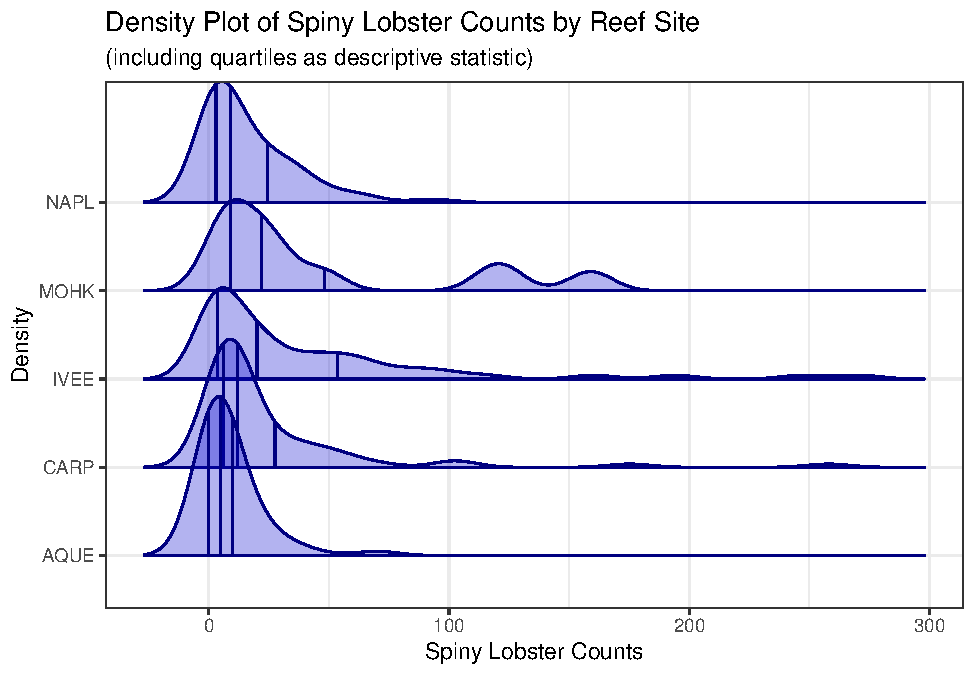
\includegraphics{hw1-lobstrs-eds241_files/figure-latex/unnamed-chunk-5-1.pdf}

\begin{Shaded}
\begin{Highlighting}[]
\CommentTok{\# plot 2: beeswarm (with boxplot)}

\NormalTok{plot2 }\OtherTok{\textless{}{-}} \FunctionTok{ggplot}\NormalTok{(spiny\_counts, }\FunctionTok{aes}\NormalTok{(}\AttributeTok{x =}\NormalTok{ mpa, }\AttributeTok{y =}\NormalTok{ counts)) }\SpecialCharTok{+}
    \FunctionTok{geom\_boxplot}\NormalTok{(}\AttributeTok{outlier.shape =} \ConstantTok{NA}\NormalTok{) }\SpecialCharTok{+}
\NormalTok{    ggbeeswarm}\SpecialCharTok{::}\FunctionTok{geom\_beeswarm}\NormalTok{(}\AttributeTok{size =} \DecValTok{1}\NormalTok{, }\AttributeTok{alpha =}\NormalTok{ .}\DecValTok{4}\NormalTok{, }\AttributeTok{color =} \StringTok{"orange4"}\NormalTok{) }\SpecialCharTok{+}
    \FunctionTok{scale\_y\_continuous}\NormalTok{(}\AttributeTok{limits =} \FunctionTok{quantile}\NormalTok{(spiny\_counts}\SpecialCharTok{$}\NormalTok{counts, }\FunctionTok{c}\NormalTok{(}\FloatTok{0.1}\NormalTok{, }\FloatTok{0.9}\NormalTok{))) }\SpecialCharTok{+}
    \FunctionTok{theme\_bw}\NormalTok{() }\SpecialCharTok{+}
    \FunctionTok{labs}\NormalTok{(}
        \AttributeTok{title =} \StringTok{"Boxplot with Beeswarm Overlay of Spiny Lobster Counts by MPA Status"}\NormalTok{,}
        \AttributeTok{x =} \StringTok{"MPA Status"}\NormalTok{,}
        \AttributeTok{y =} \StringTok{"Lobster Counts"}\NormalTok{) }
\FunctionTok{print}\NormalTok{(plot2)   }
\end{Highlighting}
\end{Shaded}

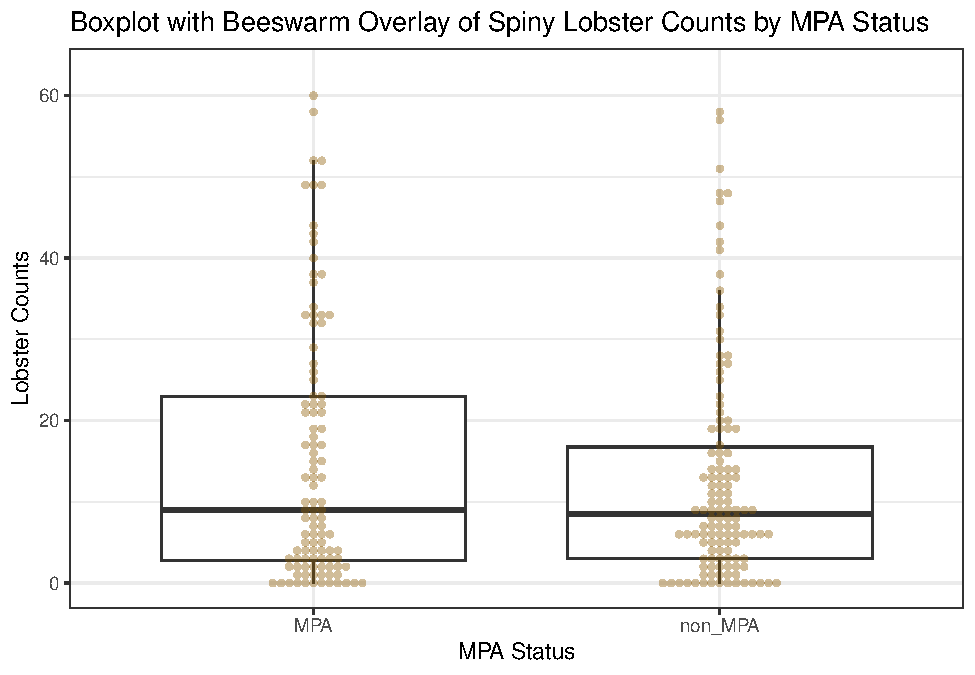
\includegraphics{hw1-lobstrs-eds241_files/figure-latex/unnamed-chunk-5-2.pdf}

\begin{Shaded}
\begin{Highlighting}[]
\CommentTok{\# plot 3: violin plot}

\NormalTok{plot3 }\OtherTok{\textless{}{-}} \FunctionTok{ggplot}\NormalTok{(spiny\_counts, }\FunctionTok{aes}\NormalTok{(}\AttributeTok{x =} \FunctionTok{as.factor}\NormalTok{(year), }\AttributeTok{y =}\NormalTok{ counts)) }\SpecialCharTok{+}
    \FunctionTok{geom\_violin}\NormalTok{(}\AttributeTok{color =} \StringTok{"green4"}\NormalTok{, }\AttributeTok{fill =} \StringTok{"green3"}\NormalTok{) }\SpecialCharTok{+}
    \FunctionTok{stat\_summary}\NormalTok{(}\AttributeTok{fun.y=}\NormalTok{median, }\AttributeTok{geom=}\StringTok{"crossbar"}\NormalTok{, }\AttributeTok{size=}\NormalTok{.}\DecValTok{3}\NormalTok{, }\AttributeTok{color=}\StringTok{"black"}\NormalTok{) }\SpecialCharTok{+}
    \FunctionTok{scale\_y\_continuous}\NormalTok{(}\AttributeTok{limits =} \FunctionTok{quantile}\NormalTok{(spiny\_counts}\SpecialCharTok{$}\NormalTok{counts, }\FunctionTok{c}\NormalTok{(}\FloatTok{0.1}\NormalTok{, }\FloatTok{0.9}\NormalTok{))) }\SpecialCharTok{+}
    \FunctionTok{theme\_bw}\NormalTok{() }\SpecialCharTok{+}
    \FunctionTok{labs}\NormalTok{(}
        \AttributeTok{title =} \StringTok{"Violin Plot of Spiny Lobster Counts by Year (2012{-}2018)"}\NormalTok{,}
        \AttributeTok{subtitle =} \StringTok{"(including medians as the descriptive statistic)"}\NormalTok{,}
        \AttributeTok{x =} \StringTok{"Year"}\NormalTok{,}
        \AttributeTok{y =} \StringTok{"Spiny Lobster Counts"}\NormalTok{)}

\FunctionTok{print}\NormalTok{(plot3)}
\end{Highlighting}
\end{Shaded}

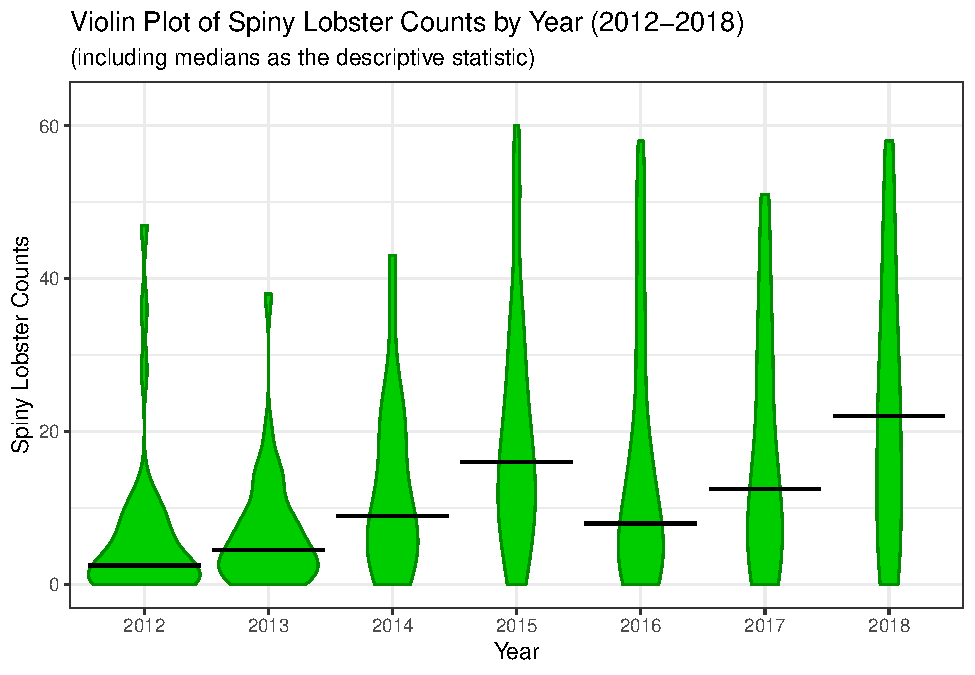
\includegraphics{hw1-lobstrs-eds241_files/figure-latex/unnamed-chunk-5-3.pdf}

\begin{Shaded}
\begin{Highlighting}[]
\CommentTok{\# plot 4: jitter plot}

\NormalTok{plot4 }\OtherTok{\textless{}{-}} \FunctionTok{ggplot}\NormalTok{(spiny\_counts, }\FunctionTok{aes}\NormalTok{(}\AttributeTok{x =}\NormalTok{ year, }\AttributeTok{y =}\NormalTok{ mean\_size)) }\SpecialCharTok{+}
    \FunctionTok{geom\_jitter}\NormalTok{(}\AttributeTok{color =} \StringTok{"darkred"}\NormalTok{, }\AttributeTok{size =} \FloatTok{1.2}\NormalTok{) }\SpecialCharTok{+}
    \FunctionTok{theme\_bw}\NormalTok{() }\SpecialCharTok{+}
    \FunctionTok{labs}\NormalTok{(}
        \AttributeTok{title =} \StringTok{"Jitter Plot of Spiny Lobster Average Size by Year (2012 {-} 2018)"}\NormalTok{,}
        \AttributeTok{x =} \StringTok{"Year"}\NormalTok{,}
        \AttributeTok{y =} \StringTok{"Average Lobster Size"}\NormalTok{) }\SpecialCharTok{+}
     \FunctionTok{scale\_x\_continuous}\NormalTok{(}\AttributeTok{limits=}\FunctionTok{c}\NormalTok{(}\DecValTok{2012}\NormalTok{, }\DecValTok{2018}\NormalTok{), }\AttributeTok{expand =} \FunctionTok{c}\NormalTok{(}\DecValTok{0}\NormalTok{,}\ConstantTok{NA}\NormalTok{))}
    

\FunctionTok{print}\NormalTok{(plot4)}
\end{Highlighting}
\end{Shaded}

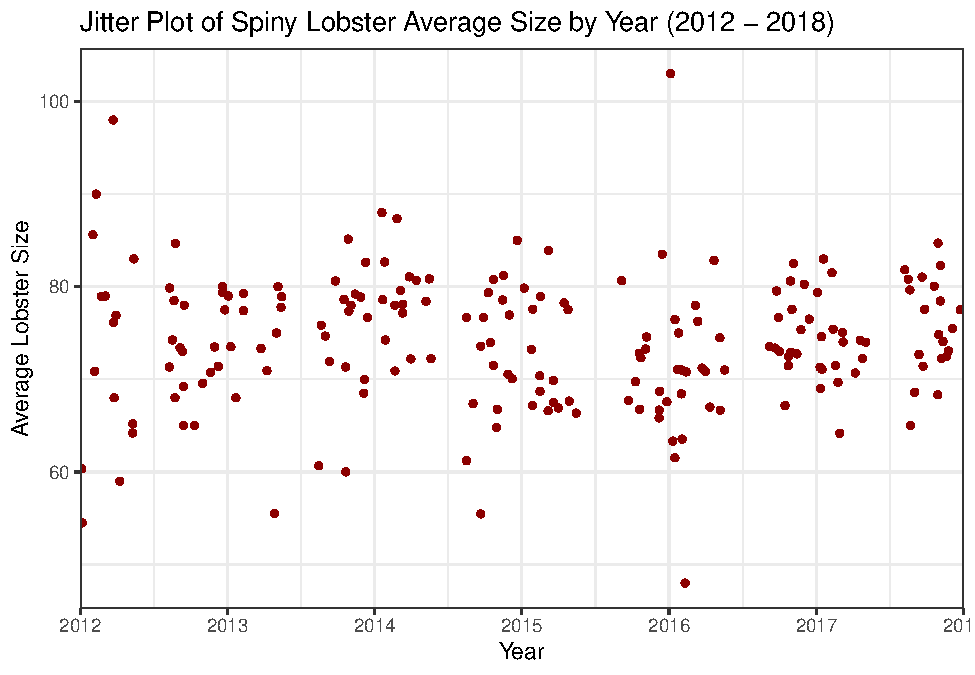
\includegraphics{hw1-lobstrs-eds241_files/figure-latex/unnamed-chunk-5-4.pdf}

\textbf{c.} Compare means of the outcome by treatment group. Using the
\texttt{tbl\_summary()} function from the package
\href{https://www.danieldsjoberg.com/gtsummary/articles/tbl_summary.html}{\texttt{gt\_summary}}

\begin{Shaded}
\begin{Highlighting}[]
\CommentTok{\# USE: gt\_summary::tbl\_summary()}

\NormalTok{spiny\_counts }\SpecialCharTok{|\textgreater{}} 
\NormalTok{    dplyr}\SpecialCharTok{::}\FunctionTok{select}\NormalTok{(counts, mean\_size, mpa) }\SpecialCharTok{|\textgreater{}}
    \FunctionTok{tbl\_summary}\NormalTok{(}\AttributeTok{by =}\NormalTok{ mpa,}
                \AttributeTok{statistic =} \FunctionTok{list}\NormalTok{(}\FunctionTok{all\_continuous}\NormalTok{() }\SpecialCharTok{\textasciitilde{}} \StringTok{"\{mean\}"}\NormalTok{)) }\SpecialCharTok{|\textgreater{}}
    \FunctionTok{modify\_caption}\NormalTok{(}\StringTok{"**Comparing the mean counts and mean sizes of California Spiny Lobsters at MPA and non{-}MPA sites**"}\NormalTok{)}
\end{Highlighting}
\end{Shaded}

\begin{table}[!t]
\caption{\label{tab:unnamed-chunk-6}\textbf{Comparing the mean counts and mean sizes of California Spiny Lobsters at MPA and non-MPA sites}} 
\fontsize{12.0pt}{14.4pt}\selectfont
\begin{tabular*}{\linewidth}{@{\extracolsep{\fill}}lcc}
\toprule
\textbf{Characteristic} & \textbf{MPA}  N = 119\textsuperscript{\textit{1}} & \textbf{non\_MPA}  N = 133\textsuperscript{\textit{1}} \\ 
\midrule\addlinespace[2.5pt]
site &  &  \\ 
    AQUE & 0 (0\%) & 49 (37\%) \\ 
    CARP & 0 (0\%) & 63 (47\%) \\ 
    IVEE & 56 (47\%) & 0 (0\%) \\ 
    MOHK & 0 (0\%) & 21 (16\%) \\ 
    NAPL & 63 (53\%) & 0 (0\%) \\ 
year &  &  \\ 
    2012 & 17 (14\%) & 19 (14\%) \\ 
    2013 & 17 (14\%) & 19 (14\%) \\ 
    2014 & 17 (14\%) & 19 (14\%) \\ 
    2015 & 17 (14\%) & 19 (14\%) \\ 
    2016 & 17 (14\%) & 19 (14\%) \\ 
    2017 & 17 (14\%) & 19 (14\%) \\ 
    2018 & 17 (14\%) & 19 (14\%) \\ 
counts & 28 & 23 \\ 
mean\_size & 76 & 73 \\ 
    Unknown & 12 & 15 \\ 
\bottomrule
\end{tabular*}
\begin{minipage}{\linewidth}
\textsuperscript{\textit{1}}n (\%); Mean\\
\end{minipage}
\end{table}

\begin{center}\rule{0.5\linewidth}{0.5pt}\end{center}

Step 4: OLS regression- building intuition

\textbf{a.} Start with a simple OLS estimator of lobster counts
regressed on treatment. Use the function \texttt{summ()} from the
\href{https://jtools.jacob-long.com/}{\texttt{jtools}} package to print
the OLS output

\textbf{b.} Interpret the intercept \& predictor coefficients \emph{in
your own words}. Use full sentences and write your interpretation of the
regression results to be as clear as possible to a non-academic
audience.

\begin{Shaded}
\begin{Highlighting}[]
\CommentTok{\# }\AlertTok{NOTE}\CommentTok{: We will not evaluate/interpret model fit in this assignment (e.g., R{-}square)}

\NormalTok{m1\_ols }\OtherTok{\textless{}{-}} \FunctionTok{lm}\NormalTok{(counts }\SpecialCharTok{\textasciitilde{}}\NormalTok{ treat, }\AttributeTok{data =}\NormalTok{ spiny\_counts)}

\FunctionTok{summ}\NormalTok{(m1\_ols, }\AttributeTok{model.fit =} \ConstantTok{FALSE}\NormalTok{) }
\end{Highlighting}
\end{Shaded}

\begin{table}[!h]
\centering
\begin{tabular}{lr}
\toprule
\cellcolor{gray!10}{Observations} & \cellcolor{gray!10}{252}\\
Dependent variable & counts\\
\cellcolor{gray!10}{Type} & \cellcolor{gray!10}{OLS linear regression}\\
\bottomrule
\end{tabular}
\end{table}  \begin{table}[!h]
\centering
\begin{threeparttable}
\begin{tabular}{lrrrr}
\toprule
  & Est. & S.E. & t val. & p\\
\midrule
\cellcolor{gray!10}{(Intercept)} & \cellcolor{gray!10}{22.73} & \cellcolor{gray!10}{3.57} & \cellcolor{gray!10}{6.36} & \cellcolor{gray!10}{0.00}\\
treat & 5.36 & 5.20 & 1.03 & 0.30\\
\bottomrule
\end{tabular}
\begin{tablenotes}
\item Standard errors: OLS
\end{tablenotes}
\end{threeparttable}
\end{table}

The intercept coefficient is the lobster count when the site is not an
MPA (22.73). The treatment plus the intercept is the count when the site
is an MPA (28.09). The p-value of the intercept is 0, which is means it
is significant. The treat coefficient has a p value of .3, meaning that
the coefficient is not statistically significant.

\textbf{c.} Check the model assumptions using the \texttt{check\_model}
function from the \texttt{performance} package

\textbf{d.} Explain the results of the 4 diagnostic plots. Why are we
getting this result?

\begin{Shaded}
\begin{Highlighting}[]
\FunctionTok{print}\NormalTok{(}\FunctionTok{check\_model}\NormalTok{(m1\_ols,  }\AttributeTok{check =} \StringTok{"qq"}\NormalTok{ ))}
\end{Highlighting}
\end{Shaded}

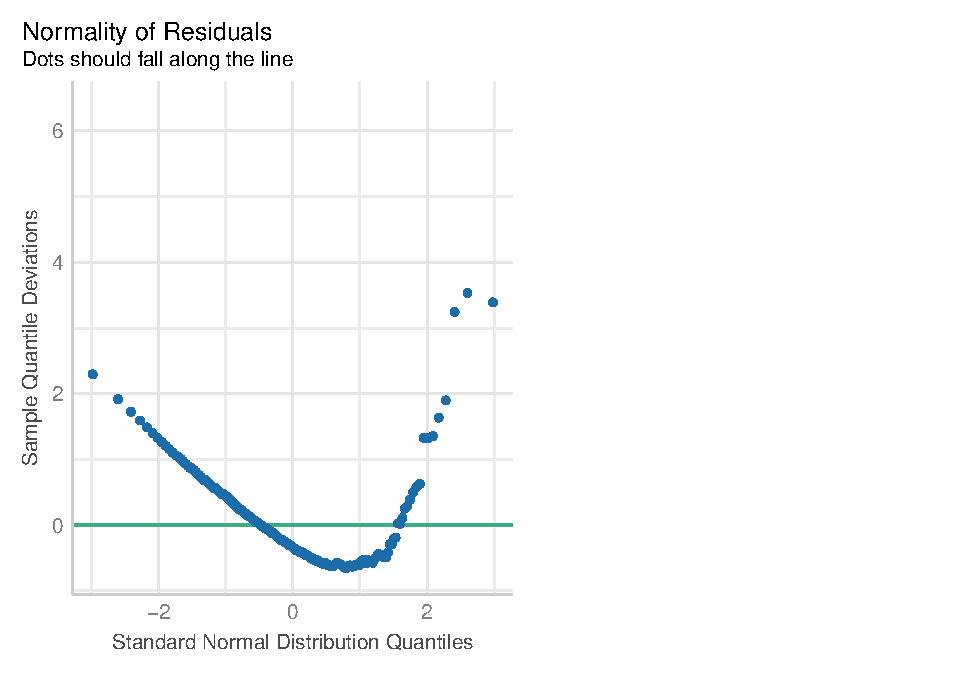
\includegraphics{hw1-lobstrs-eds241_files/figure-latex/unnamed-chunk-8-1.pdf}

This model check is looking at the normality of residuals. If our
residuals were normal, the dots would fall along the green line. Our
results mean that are residuals are very much not normal. Because we are
using a linear regression model, it's important that our residuals are
normal. Our results show that our OLS model is not a good fit.

\begin{Shaded}
\begin{Highlighting}[]
\FunctionTok{print}\NormalTok{(}\FunctionTok{check\_model}\NormalTok{(m1\_ols, }\AttributeTok{check =} \StringTok{"normality"}\NormalTok{))}
\end{Highlighting}
\end{Shaded}

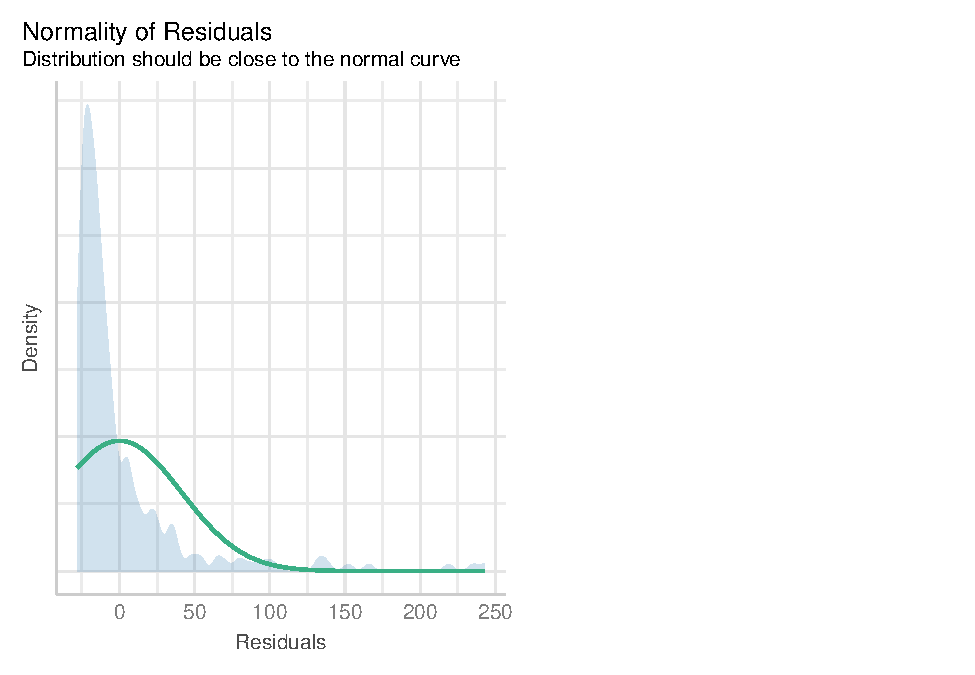
\includegraphics{hw1-lobstrs-eds241_files/figure-latex/unnamed-chunk-9-1.pdf}

This model is also looking at the normality of residuals, this time
looking at the shape of the curve. If our distributions fell close to
the green curve on the graph, we would have a normally distributed curve
as expected if our model was linear. Because it's far from being close
to the curve, it's clear our distribution is not normal and we should
not be using a linear regression model.

\begin{Shaded}
\begin{Highlighting}[]
\FunctionTok{print}\NormalTok{(}\FunctionTok{check\_model}\NormalTok{(m1\_ols, }\AttributeTok{check =} \StringTok{"homogeneity"}\NormalTok{))}
\end{Highlighting}
\end{Shaded}

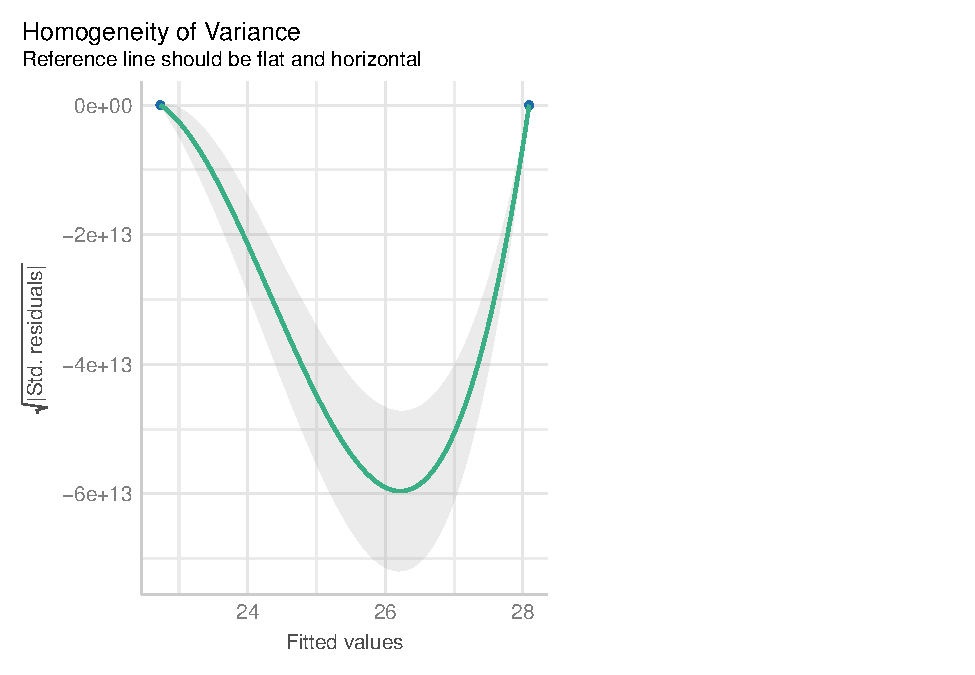
\includegraphics{hw1-lobstrs-eds241_files/figure-latex/unnamed-chunk-10-1.pdf}

This model is looking at the homogeneity of variance, meaning that we're
looking at the equality of the variance across our samples. The subtitle
tells us that the reference line should be flat and horizontal, but when
we look at the graph we can tell that the line is extremely curved in a
U shape. This is a sign that our data could be skewed or biased. This is
another sign that a linear regression is not the right choice.

\begin{Shaded}
\begin{Highlighting}[]
\FunctionTok{print}\NormalTok{(}\FunctionTok{check\_model}\NormalTok{(m1\_ols, }\AttributeTok{check =} \StringTok{"pp\_check"}\NormalTok{))}
\end{Highlighting}
\end{Shaded}

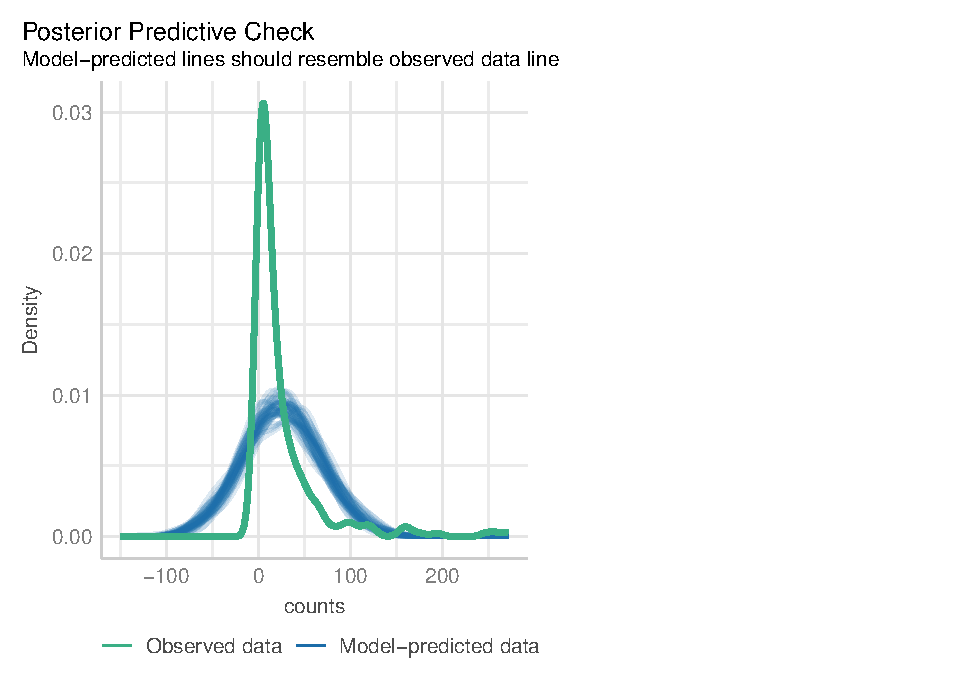
\includegraphics{hw1-lobstrs-eds241_files/figure-latex/unnamed-chunk-11-1.pdf}

This model is looking at the posterior predictive check, meaning that
it's looking at how well the model shows means, standard deviations, and
quantiles. If the model predicted data lines lined up with the green
observed data line, our model would successfully capture relevant
aspects. We are seeing that our lines are not lining up because our
model is not showing these aspects successfully. This is another sign
that our linear regression model is not the right choice.

\begin{center}\rule{0.5\linewidth}{0.5pt}\end{center}

Step 5: Fitting GLMs

\textbf{a.} Estimate a Poisson regression model using the \texttt{glm()}
function

\textbf{b.} Interpret the predictor coefficient in your own words. Use
full sentences and write your interpretation of the results to be as
clear as possible to a non-academic audience.

\textbf{c.} Explain the statistical concept of dispersion and
overdispersion in the context of this model.

\textbf{d.} Compare results with previous model, explain change in the
significance of the treatment effect

\begin{Shaded}
\begin{Highlighting}[]
\CommentTok{\#HINT1: Incidence Ratio Rate (IRR): Exponentiation of beta returns coefficient which is interpreted as the \textquotesingle{}percent change\textquotesingle{} for a one unit increase in the predictor }

\CommentTok{\#HINT2: For the second glm() argument \textasciigrave{}family\textasciigrave{} use the following specification option \textasciigrave{}family = poisson(link = "log")\textasciigrave{}}

\NormalTok{m2\_pois }\OtherTok{\textless{}{-}} \FunctionTok{glm}\NormalTok{(counts }\SpecialCharTok{\textasciitilde{}}\NormalTok{ treat,}
\NormalTok{               spiny\_counts,}
               \AttributeTok{family =} \FunctionTok{poisson}\NormalTok{(}\AttributeTok{link =} \StringTok{"log"}\NormalTok{))}

\FunctionTok{summ}\NormalTok{(m2\_pois)}
\end{Highlighting}
\end{Shaded}

\begin{table}[!h]
\centering
\begin{tabular}{lr}
\toprule
\cellcolor{gray!10}{Observations} & \cellcolor{gray!10}{252}\\
Dependent variable & counts\\
\cellcolor{gray!10}{Type} & \cellcolor{gray!10}{Generalized linear model}\\
Family & poisson\\
\cellcolor{gray!10}{Link} & \cellcolor{gray!10}{log}\\
\bottomrule
\end{tabular}
\end{table} \begin{table}[!h]
\centering
\begin{tabular}{lr}
\toprule
\cellcolor{gray!10}{$\chi^2$(1)} & \cellcolor{gray!10}{71.36}\\
p & 0.00\\
\cellcolor{gray!10}{Pseudo-R² (Cragg-Uhler)} & \cellcolor{gray!10}{0.25}\\
Pseudo-R² (McFadden) & 0.01\\
\cellcolor{gray!10}{AIC} & \cellcolor{gray!10}{11365.62}\\
\addlinespace
BIC & 11372.68\\
\bottomrule
\end{tabular}
\end{table} \begin{table}[!h]
\centering
\begin{threeparttable}
\begin{tabular}{lrrrr}
\toprule
  & Est. & S.E. & z val. & p\\
\midrule
\cellcolor{gray!10}{(Intercept)} & \cellcolor{gray!10}{3.12} & \cellcolor{gray!10}{0.02} & \cellcolor{gray!10}{171.74} & \cellcolor{gray!10}{0.00}\\
treat & 0.21 & 0.03 & 8.44 & 0.00\\
\bottomrule
\end{tabular}
\begin{tablenotes}
\item Standard errors: MLE
\end{tablenotes}
\end{threeparttable}
\end{table}

\begin{Shaded}
\begin{Highlighting}[]
\FunctionTok{print}\NormalTok{(}\FunctionTok{exp}\NormalTok{(.}\DecValTok{21}\NormalTok{) }\SpecialCharTok{{-}} \DecValTok{1}\NormalTok{)}
\end{Highlighting}
\end{Shaded}

\begin{verbatim}
## [1] 0.2336781
\end{verbatim}

\begin{enumerate}
\def\labelenumi{\alph{enumi}.}
\setcounter{enumi}{1}
\item
  The predictor coefficient is .21 on a log scale. When using a poisson
  regression model we take the exponent of that predictor coefficient
  and then subtract one. This gives us the percent changed when the
  treatment is present (it is an mpa site). The results are a 23.36
  percent increase.
\item
  The poisson model makes the assumption that the mean is equal to the
  dispersion (variance). When there is overdispersion that means that
  the dispersion (variance) is greater than the mean.
\item
  In the previous model, the treatment effect was not statistically
  significant. Its p-value was .3, which is over the .05 threshold for
  significance. In this model, the p-value of the treatment is 0.00,
  meaning that it is significant in this model. In the previous model,
  the treatment effect was 5.36, translating to about a 23.58 percent
  increase from non-mpa sites. In this model the predictor coefficient
  tells us that the treament effect is 23.36 percent. Both results are
  extremely close, although there is a slight increase in signficance of
  effect in the poisson model.
\end{enumerate}

\textbf{e.} Check the model assumptions. Explain results.

The model assumes that the mean is equal to the distribution. By using
the overdispersion test we can tell that the dispersion does not equal
the mean, meaning that poisson is not a good fit. We also checked the
zero inflation, which showed that there were too many zeros in our
model, another sign that poisson is not a good fit.

\textbf{f.} Conduct tests for over-dispersion \& zero-inflation. Explain
results.

\begin{Shaded}
\begin{Highlighting}[]
\FunctionTok{print}\NormalTok{(}\FunctionTok{check\_model}\NormalTok{(m2\_pois))}
\end{Highlighting}
\end{Shaded}

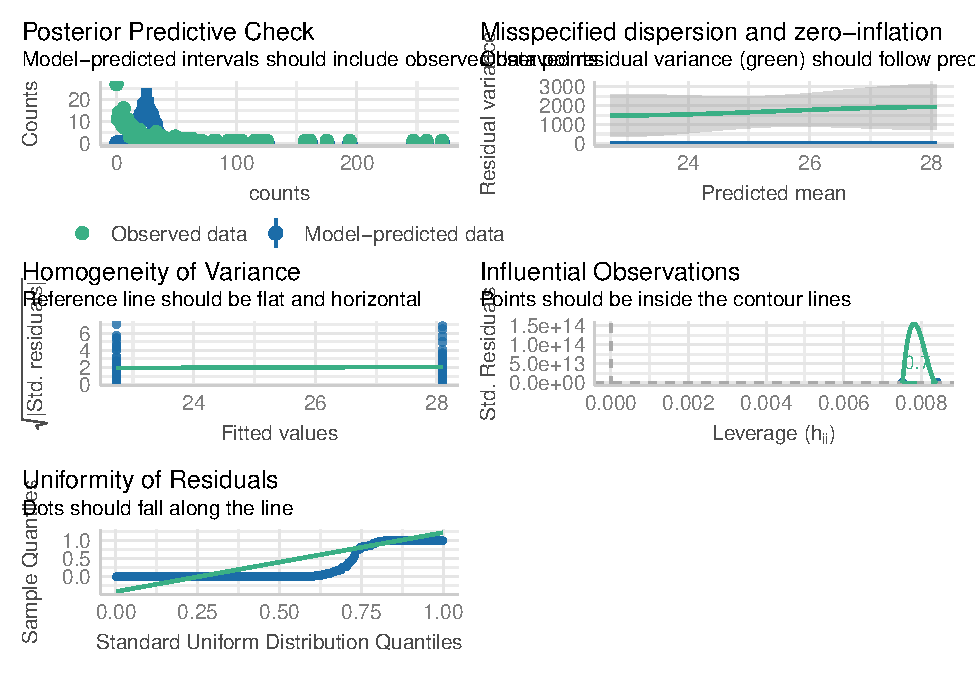
\includegraphics{hw1-lobstrs-eds241_files/figure-latex/unnamed-chunk-13-1.pdf}

\begin{Shaded}
\begin{Highlighting}[]
\FunctionTok{print}\NormalTok{(}\FunctionTok{check\_overdispersion}\NormalTok{(m2\_pois))}
\end{Highlighting}
\end{Shaded}

\begin{verbatim}
## # Overdispersion test
## 
##        dispersion ratio =    67.033
##   Pearson's Chi-Squared = 16758.289
##                 p-value =   < 0.001
\end{verbatim}

This test shows that overdispersion was detected in the model. The
p-value is less than .001, meaning that the test results are
statistically significant. We now know that the dispersion is greater
than the mean.

\begin{Shaded}
\begin{Highlighting}[]
\FunctionTok{print}\NormalTok{(}\FunctionTok{check\_zeroinflation}\NormalTok{(m2\_pois))}
\end{Highlighting}
\end{Shaded}

\begin{verbatim}
## # Check for zero-inflation
## 
##    Observed zeros: 27
##   Predicted zeros: 0
##             Ratio: 0.00
\end{verbatim}

This test shows us that the model is underfitting zeros and that
zero-inflation is probable. That means that the model is allowing too
many zeros. This is a sign to us that a glm model was not the right
choice.

\textbf{g.} Fit a negative binomial model using the function glm.nb()
from the package \texttt{MASS} and check model diagnostics

\textbf{h.} In 1-2 sentences explain rationale for fitting this GLM
model.

\textbf{i.} Interpret the treatment estimate result in your own words.
Compare with results from the previous model.

\begin{Shaded}
\begin{Highlighting}[]
\CommentTok{\# }\AlertTok{NOTE}\CommentTok{: The \textasciigrave{}glm.nb()\textasciigrave{} function does not require a \textasciigrave{}family\textasciigrave{} argument}

\NormalTok{m3\_nb }\OtherTok{\textless{}{-}}\NormalTok{ MASS}\SpecialCharTok{::}\FunctionTok{glm.nb}\NormalTok{(counts }\SpecialCharTok{\textasciitilde{}}\NormalTok{ treat,}
\NormalTok{               spiny\_counts)}

\FunctionTok{summ}\NormalTok{(m3\_nb)}
\end{Highlighting}
\end{Shaded}

\begin{table}[!h]
\centering
\begin{tabular}{lr}
\toprule
\cellcolor{gray!10}{Observations} & \cellcolor{gray!10}{252}\\
Dependent variable & counts\\
\cellcolor{gray!10}{Type} & \cellcolor{gray!10}{Generalized linear model}\\
Family & Negative Binomial(0.55)\\
\cellcolor{gray!10}{Link} & \cellcolor{gray!10}{log}\\
\bottomrule
\end{tabular}
\end{table} \begin{table}[!h]
\centering
\begin{tabular}{lr}
\toprule
\cellcolor{gray!10}{$\chi^2$(250)} & \cellcolor{gray!10}{1.52}\\
p & 0.22\\
\cellcolor{gray!10}{Pseudo-R² (Cragg-Uhler)} & \cellcolor{gray!10}{0.01}\\
Pseudo-R² (McFadden) & 0.00\\
\cellcolor{gray!10}{AIC} & \cellcolor{gray!10}{2088.53}\\
\addlinespace
BIC & 2099.12\\
\bottomrule
\end{tabular}
\end{table} \begin{table}[!h]
\centering
\begin{threeparttable}
\begin{tabular}{lrrrr}
\toprule
  & Est. & S.E. & z val. & p\\
\midrule
\cellcolor{gray!10}{(Intercept)} & \cellcolor{gray!10}{3.12} & \cellcolor{gray!10}{0.12} & \cellcolor{gray!10}{26.40} & \cellcolor{gray!10}{0.00}\\
treat & 0.21 & 0.17 & 1.23 & 0.22\\
\bottomrule
\end{tabular}
\begin{tablenotes}
\item Standard errors: MLE
\end{tablenotes}
\end{threeparttable}
\end{table}

\begin{Shaded}
\begin{Highlighting}[]
\FunctionTok{print}\NormalTok{(}\FunctionTok{exp}\NormalTok{(.}\DecValTok{21}\NormalTok{) }\SpecialCharTok{{-}} \DecValTok{1}\NormalTok{)}
\end{Highlighting}
\end{Shaded}

\begin{verbatim}
## [1] 0.2336781
\end{verbatim}

\begin{Shaded}
\begin{Highlighting}[]
\FunctionTok{print}\NormalTok{(}\FunctionTok{check\_overdispersion}\NormalTok{(m3\_nb))}
\end{Highlighting}
\end{Shaded}

\begin{verbatim}
## # Overdispersion test
## 
##  dispersion ratio = 1.398
##           p-value = 0.088
\end{verbatim}

As expected, this model controls for overdispersion, so there is none
present.

\begin{Shaded}
\begin{Highlighting}[]
\FunctionTok{print}\NormalTok{(}\FunctionTok{check\_zeroinflation}\NormalTok{(m3\_nb))}
\end{Highlighting}
\end{Shaded}

\begin{verbatim}
## # Check for zero-inflation
## 
##    Observed zeros: 27
##   Predicted zeros: 30
##             Ratio: 1.12
\end{verbatim}

This model does not control/ have a parameter for zero inflation, so it
makes sense that overfitting of zeros would still be present.

\begin{Shaded}
\begin{Highlighting}[]
\FunctionTok{print}\NormalTok{(}\FunctionTok{check\_predictions}\NormalTok{(m3\_nb))}
\end{Highlighting}
\end{Shaded}

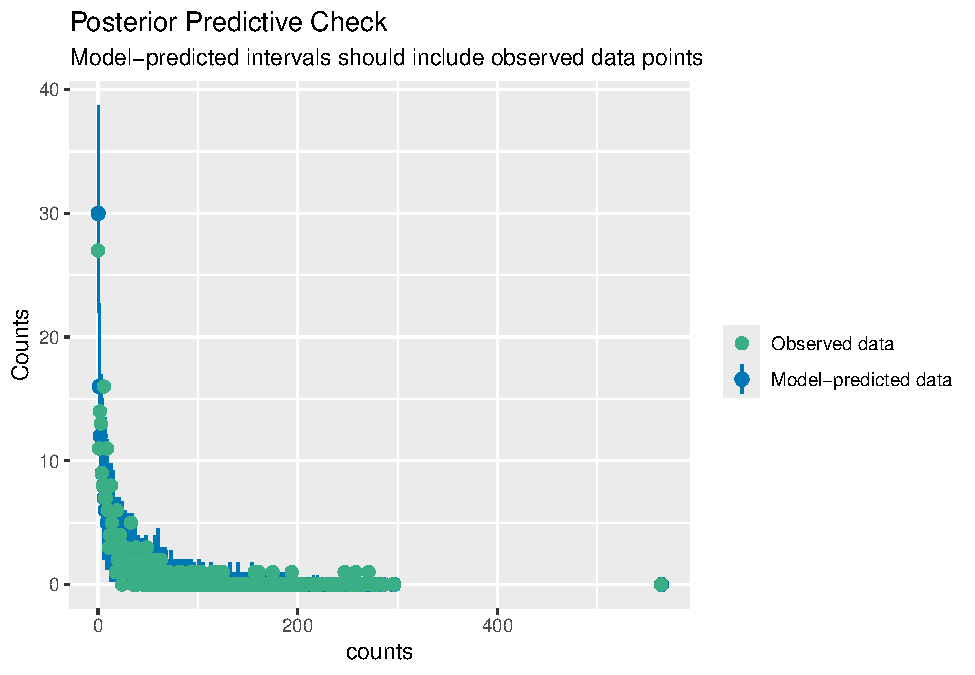
\includegraphics{hw1-lobstrs-eds241_files/figure-latex/unnamed-chunk-19-1.pdf}

This model's observed data and model-predicted data seem to line up in
the graph. Meaning that the model represents mean, quantiles, and
standard deviation well.

\begin{Shaded}
\begin{Highlighting}[]
\FunctionTok{print}\NormalTok{(}\FunctionTok{check\_model}\NormalTok{(m3\_nb))}
\end{Highlighting}
\end{Shaded}

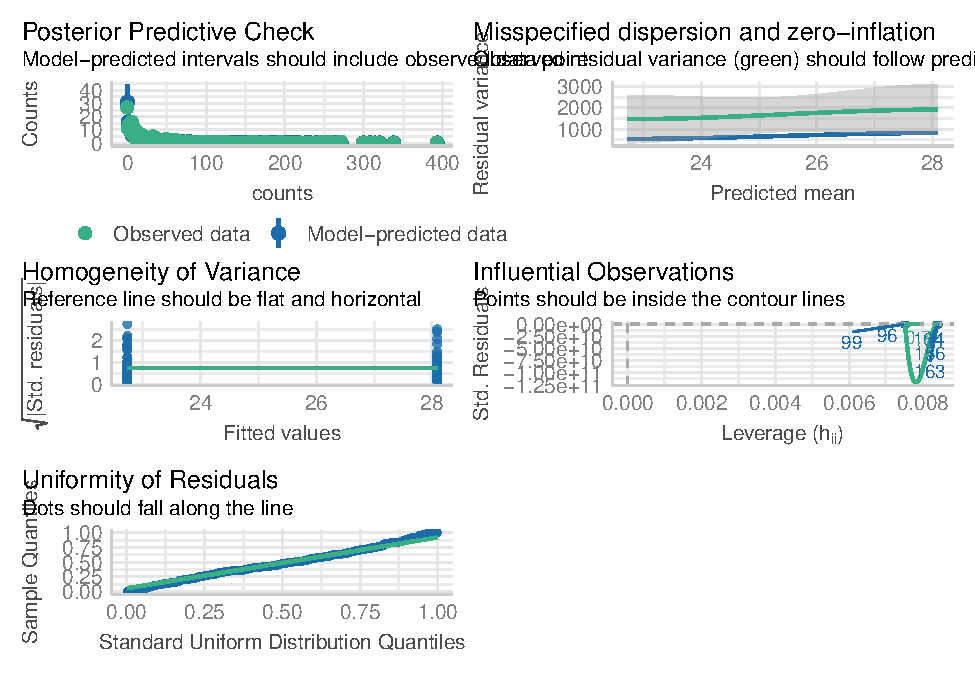
\includegraphics{hw1-lobstrs-eds241_files/figure-latex/unnamed-chunk-20-1.pdf}

\begin{enumerate}
\def\labelenumi{\alph{enumi}.}
\setcounter{enumi}{7}
\item
  The rationale for fitting a negative binomial model is that it
  accounts for over dispersion by adding a parameter. We know from the
  poisson model checks that there is over dispersion in our model, so we
  know that over dispersion is something we need to account for.
\item
  The treatment estimate is .21, and similar to the poisson model this
  one also shows log-scale coefficients. When performing the equation we
  can tell that the treatment effect is 23.36 percent. The p-value of
  the treatment coefficient is .22, meaning it's not statistically
  significant. The treatment effect is very similar to the first model
  (23.58), and the same as the poisson model (23.36)
\end{enumerate}

\begin{center}\rule{0.5\linewidth}{0.5pt}\end{center}

Step 6: Compare models

\textbf{a.} Use the \texttt{export\_summ()} function from the
\texttt{jtools} package to look at the three regression models you fit
side-by-side.

\textbf{c.} Write a short paragraph comparing the results. Is the
treatment effect \texttt{robust} or stable across the model
specifications.

\begin{Shaded}
\begin{Highlighting}[]
\FunctionTok{export\_summs}\NormalTok{(m1\_ols, m2\_pois, m3\_nb,}
             \AttributeTok{model.names =} \FunctionTok{c}\NormalTok{(}\StringTok{"OLS"}\NormalTok{,}\StringTok{"Poisson"}\NormalTok{, }\StringTok{"NB"}\NormalTok{))}
\end{Highlighting}
\end{Shaded}

 
  \providecommand{\huxb}[2]{\arrayrulecolor[RGB]{#1}\global\arrayrulewidth=#2pt}
  \providecommand{\huxvb}[2]{\color[RGB]{#1}\vrule width #2pt}
  \providecommand{\huxtpad}[1]{\rule{0pt}{#1}}
  \providecommand{\huxbpad}[1]{\rule[-#1]{0pt}{#1}}

\begin{table}[ht]
\begin{centerbox}
\begin{threeparttable}
 \setlength{\tabcolsep}{0pt}
\begin{tabular}{l l l l}


\hhline{>{\huxb{0, 0, 0}{0.8}}->{\huxb{0, 0, 0}{0.8}}->{\huxb{0, 0, 0}{0.8}}->{\huxb{0, 0, 0}{0.8}}-}
\arrayrulecolor{black}

\multicolumn{1}{!{\huxvb{0, 0, 0}{0}}c!{\huxvb{0, 0, 0}{0}}}{\huxtpad{6pt + 1em}\centering \hspace{6pt}  \hspace{6pt}\huxbpad{6pt}} &
\multicolumn{1}{c!{\huxvb{0, 0, 0}{0}}}{\huxtpad{6pt + 1em}\centering \hspace{6pt} OLS \hspace{6pt}\huxbpad{6pt}} &
\multicolumn{1}{c!{\huxvb{0, 0, 0}{0}}}{\huxtpad{6pt + 1em}\centering \hspace{6pt} Poisson \hspace{6pt}\huxbpad{6pt}} &
\multicolumn{1}{c!{\huxvb{0, 0, 0}{0}}}{\huxtpad{6pt + 1em}\centering \hspace{6pt} NB \hspace{6pt}\huxbpad{6pt}} \tabularnewline[-0.5pt]


\hhline{>{\huxb{255, 255, 255}{0.4}}->{\huxb{0, 0, 0}{0.4}}->{\huxb{0, 0, 0}{0.4}}->{\huxb{0, 0, 0}{0.4}}-}
\arrayrulecolor{black}

\multicolumn{1}{!{\huxvb{0, 0, 0}{0}}l!{\huxvb{0, 0, 0}{0}}}{\huxtpad{6pt + 1em}\raggedright \hspace{6pt} (Intercept) \hspace{6pt}\huxbpad{6pt}} &
\multicolumn{1}{r!{\huxvb{0, 0, 0}{0}}}{\huxtpad{6pt + 1em}\raggedleft \hspace{6pt} 22.73 *** \hspace{6pt}\huxbpad{6pt}} &
\multicolumn{1}{r!{\huxvb{0, 0, 0}{0}}}{\huxtpad{6pt + 1em}\raggedleft \hspace{6pt} 3.12 *** \hspace{6pt}\huxbpad{6pt}} &
\multicolumn{1}{r!{\huxvb{0, 0, 0}{0}}}{\huxtpad{6pt + 1em}\raggedleft \hspace{6pt} 3.12 *** \hspace{6pt}\huxbpad{6pt}} \tabularnewline[-0.5pt]


\hhline{}
\arrayrulecolor{black}

\multicolumn{1}{!{\huxvb{0, 0, 0}{0}}l!{\huxvb{0, 0, 0}{0}}}{\huxtpad{6pt + 1em}\raggedright \hspace{6pt}  \hspace{6pt}\huxbpad{6pt}} &
\multicolumn{1}{r!{\huxvb{0, 0, 0}{0}}}{\huxtpad{6pt + 1em}\raggedleft \hspace{6pt} (3.57)\hphantom{0}\hphantom{0}\hphantom{0} \hspace{6pt}\huxbpad{6pt}} &
\multicolumn{1}{r!{\huxvb{0, 0, 0}{0}}}{\huxtpad{6pt + 1em}\raggedleft \hspace{6pt} (0.02)\hphantom{0}\hphantom{0}\hphantom{0} \hspace{6pt}\huxbpad{6pt}} &
\multicolumn{1}{r!{\huxvb{0, 0, 0}{0}}}{\huxtpad{6pt + 1em}\raggedleft \hspace{6pt} (0.12)\hphantom{0}\hphantom{0}\hphantom{0} \hspace{6pt}\huxbpad{6pt}} \tabularnewline[-0.5pt]


\hhline{}
\arrayrulecolor{black}

\multicolumn{1}{!{\huxvb{0, 0, 0}{0}}l!{\huxvb{0, 0, 0}{0}}}{\huxtpad{6pt + 1em}\raggedright \hspace{6pt} treat \hspace{6pt}\huxbpad{6pt}} &
\multicolumn{1}{r!{\huxvb{0, 0, 0}{0}}}{\huxtpad{6pt + 1em}\raggedleft \hspace{6pt} 5.36\hphantom{0}\hphantom{0}\hphantom{0}\hphantom{0} \hspace{6pt}\huxbpad{6pt}} &
\multicolumn{1}{r!{\huxvb{0, 0, 0}{0}}}{\huxtpad{6pt + 1em}\raggedleft \hspace{6pt} 0.21 *** \hspace{6pt}\huxbpad{6pt}} &
\multicolumn{1}{r!{\huxvb{0, 0, 0}{0}}}{\huxtpad{6pt + 1em}\raggedleft \hspace{6pt} 0.21\hphantom{0}\hphantom{0}\hphantom{0}\hphantom{0} \hspace{6pt}\huxbpad{6pt}} \tabularnewline[-0.5pt]


\hhline{}
\arrayrulecolor{black}

\multicolumn{1}{!{\huxvb{0, 0, 0}{0}}l!{\huxvb{0, 0, 0}{0}}}{\huxtpad{6pt + 1em}\raggedright \hspace{6pt}  \hspace{6pt}\huxbpad{6pt}} &
\multicolumn{1}{r!{\huxvb{0, 0, 0}{0}}}{\huxtpad{6pt + 1em}\raggedleft \hspace{6pt} (5.20)\hphantom{0}\hphantom{0}\hphantom{0} \hspace{6pt}\huxbpad{6pt}} &
\multicolumn{1}{r!{\huxvb{0, 0, 0}{0}}}{\huxtpad{6pt + 1em}\raggedleft \hspace{6pt} (0.03)\hphantom{0}\hphantom{0}\hphantom{0} \hspace{6pt}\huxbpad{6pt}} &
\multicolumn{1}{r!{\huxvb{0, 0, 0}{0}}}{\huxtpad{6pt + 1em}\raggedleft \hspace{6pt} (0.17)\hphantom{0}\hphantom{0}\hphantom{0} \hspace{6pt}\huxbpad{6pt}} \tabularnewline[-0.5pt]


\hhline{>{\huxb{255, 255, 255}{0.4}}->{\huxb{0, 0, 0}{0.4}}->{\huxb{0, 0, 0}{0.4}}->{\huxb{0, 0, 0}{0.4}}-}
\arrayrulecolor{black}

\multicolumn{1}{!{\huxvb{0, 0, 0}{0}}l!{\huxvb{0, 0, 0}{0}}}{\huxtpad{6pt + 1em}\raggedright \hspace{6pt} N \hspace{6pt}\huxbpad{6pt}} &
\multicolumn{1}{r!{\huxvb{0, 0, 0}{0}}}{\huxtpad{6pt + 1em}\raggedleft \hspace{6pt} 252\hphantom{0}\hphantom{0}\hphantom{0}\hphantom{0}\hphantom{0}\hphantom{0}\hphantom{0} \hspace{6pt}\huxbpad{6pt}} &
\multicolumn{1}{r!{\huxvb{0, 0, 0}{0}}}{\huxtpad{6pt + 1em}\raggedleft \hspace{6pt} 252\hphantom{0}\hphantom{0}\hphantom{0}\hphantom{0}\hphantom{0}\hphantom{0}\hphantom{0} \hspace{6pt}\huxbpad{6pt}} &
\multicolumn{1}{r!{\huxvb{0, 0, 0}{0}}}{\huxtpad{6pt + 1em}\raggedleft \hspace{6pt} 252\hphantom{0}\hphantom{0}\hphantom{0}\hphantom{0}\hphantom{0}\hphantom{0}\hphantom{0} \hspace{6pt}\huxbpad{6pt}} \tabularnewline[-0.5pt]


\hhline{}
\arrayrulecolor{black}

\multicolumn{1}{!{\huxvb{0, 0, 0}{0}}l!{\huxvb{0, 0, 0}{0}}}{\huxtpad{6pt + 1em}\raggedright \hspace{6pt} R2 \hspace{6pt}\huxbpad{6pt}} &
\multicolumn{1}{r!{\huxvb{0, 0, 0}{0}}}{\huxtpad{6pt + 1em}\raggedleft \hspace{6pt} 0.00\hphantom{0}\hphantom{0}\hphantom{0}\hphantom{0} \hspace{6pt}\huxbpad{6pt}} &
\multicolumn{1}{r!{\huxvb{0, 0, 0}{0}}}{\huxtpad{6pt + 1em}\raggedleft \hspace{6pt} \hphantom{0}\hphantom{0}\hphantom{0}\hphantom{0}\hphantom{0}\hphantom{0}\hphantom{0} \hspace{6pt}\huxbpad{6pt}} &
\multicolumn{1}{r!{\huxvb{0, 0, 0}{0}}}{\huxtpad{6pt + 1em}\raggedleft \hspace{6pt} \hphantom{0}\hphantom{0}\hphantom{0}\hphantom{0}\hphantom{0}\hphantom{0}\hphantom{0} \hspace{6pt}\huxbpad{6pt}} \tabularnewline[-0.5pt]


\hhline{}
\arrayrulecolor{black}

\multicolumn{1}{!{\huxvb{0, 0, 0}{0}}l!{\huxvb{0, 0, 0}{0}}}{\huxtpad{6pt + 1em}\raggedright \hspace{6pt} AIC \hspace{6pt}\huxbpad{6pt}} &
\multicolumn{1}{r!{\huxvb{0, 0, 0}{0}}}{\huxtpad{6pt + 1em}\raggedleft \hspace{6pt} 2593.35\hphantom{0}\hphantom{0}\hphantom{0}\hphantom{0} \hspace{6pt}\huxbpad{6pt}} &
\multicolumn{1}{r!{\huxvb{0, 0, 0}{0}}}{\huxtpad{6pt + 1em}\raggedleft \hspace{6pt} 11365.62\hphantom{0}\hphantom{0}\hphantom{0}\hphantom{0} \hspace{6pt}\huxbpad{6pt}} &
\multicolumn{1}{r!{\huxvb{0, 0, 0}{0}}}{\huxtpad{6pt + 1em}\raggedleft \hspace{6pt} 2088.53\hphantom{0}\hphantom{0}\hphantom{0}\hphantom{0} \hspace{6pt}\huxbpad{6pt}} \tabularnewline[-0.5pt]


\hhline{}
\arrayrulecolor{black}

\multicolumn{1}{!{\huxvb{0, 0, 0}{0}}l!{\huxvb{0, 0, 0}{0}}}{\huxtpad{6pt + 1em}\raggedright \hspace{6pt} BIC \hspace{6pt}\huxbpad{6pt}} &
\multicolumn{1}{r!{\huxvb{0, 0, 0}{0}}}{\huxtpad{6pt + 1em}\raggedleft \hspace{6pt} 2603.94\hphantom{0}\hphantom{0}\hphantom{0}\hphantom{0} \hspace{6pt}\huxbpad{6pt}} &
\multicolumn{1}{r!{\huxvb{0, 0, 0}{0}}}{\huxtpad{6pt + 1em}\raggedleft \hspace{6pt} 11372.68\hphantom{0}\hphantom{0}\hphantom{0}\hphantom{0} \hspace{6pt}\huxbpad{6pt}} &
\multicolumn{1}{r!{\huxvb{0, 0, 0}{0}}}{\huxtpad{6pt + 1em}\raggedleft \hspace{6pt} 2099.12\hphantom{0}\hphantom{0}\hphantom{0}\hphantom{0} \hspace{6pt}\huxbpad{6pt}} \tabularnewline[-0.5pt]


\hhline{}
\arrayrulecolor{black}

\multicolumn{1}{!{\huxvb{0, 0, 0}{0}}l!{\huxvb{0, 0, 0}{0}}}{\huxtpad{6pt + 1em}\raggedright \hspace{6pt} Pseudo R2 \hspace{6pt}\huxbpad{6pt}} &
\multicolumn{1}{r!{\huxvb{0, 0, 0}{0}}}{\huxtpad{6pt + 1em}\raggedleft \hspace{6pt} \hphantom{0}\hphantom{0}\hphantom{0}\hphantom{0}\hphantom{0}\hphantom{0}\hphantom{0} \hspace{6pt}\huxbpad{6pt}} &
\multicolumn{1}{r!{\huxvb{0, 0, 0}{0}}}{\huxtpad{6pt + 1em}\raggedleft \hspace{6pt} 0.25\hphantom{0}\hphantom{0}\hphantom{0}\hphantom{0} \hspace{6pt}\huxbpad{6pt}} &
\multicolumn{1}{r!{\huxvb{0, 0, 0}{0}}}{\huxtpad{6pt + 1em}\raggedleft \hspace{6pt} 0.01\hphantom{0}\hphantom{0}\hphantom{0}\hphantom{0} \hspace{6pt}\huxbpad{6pt}} \tabularnewline[-0.5pt]


\hhline{>{\huxb{0, 0, 0}{0.8}}->{\huxb{0, 0, 0}{0.8}}->{\huxb{0, 0, 0}{0.8}}->{\huxb{0, 0, 0}{0.8}}-}
\arrayrulecolor{black}

\multicolumn{4}{!{\huxvb{0, 0, 0}{0}}l!{\huxvb{0, 0, 0}{0}}}{\huxtpad{6pt + 1em}\raggedright \hspace{6pt}  *** p $<$ 0.001;  ** p $<$ 0.01;  * p $<$ 0.05. \hspace{6pt}\huxbpad{6pt}} \tabularnewline[-0.5pt]


\hhline{}
\arrayrulecolor{black}
\end{tabular}
\end{threeparttable}\par\end{centerbox}

\end{table}
 

The results of all three models are actually quite similar. The OLS
regression looks different in numbers, but that is only because the
poisson and negative binomial are log scale coefficients. In actuality,
the treatment effect from all the models are extremely similar. The
poisson and negative binomial models have the same summary outputs. This
signifies to me that the treatment effect is robust/stable across
models.

\begin{center}\rule{0.5\linewidth}{0.5pt}\end{center}

Step 7: Building intuition - fixed effects

\textbf{a.} Create new \texttt{df} with the \texttt{year} variable
converted to a factor

\textbf{b.} Run the following OLS model using \texttt{lm()}

\begin{itemize}
\tightlist
\item
  Use the following specification for the outcome \texttt{log(counts+1)}
\item
  Estimate fixed effects for \texttt{year}
\item
  Include an interaction term between variables \texttt{treat} and
  \texttt{year}
\end{itemize}

\textbf{c.} Take a look at the regression output. Each coefficient
provides a comparison or the difference in means for a specific
sub-group in the data. Informally, describe the what the model has
estimated at a conceptual level (NOTE: you do not have to interpret
coefficients individually)

The model has estimated the treatment effect, but has also included the
years. There is a coefficient for each year for both treatment and non
treatment sites. The intercept coefficient represents the non-treatment
sites in 2012 (that's the year that is left out of the coefficients),
and the treat coefficient represents the treatment sites in 2012.

\textbf{d.} Explain why the main effect for treatment is negative? *Does
this result make sense?

This result does make sense because the main treatment effect does not
actually represent the main effect without any years, it actually
represents the treatment effect in 2012. The negative treatment
coefficient makes sense because it just means a decrease in counts in
the treatment group in 2012.

\begin{Shaded}
\begin{Highlighting}[]
\NormalTok{ff\_counts }\OtherTok{\textless{}{-}}\NormalTok{ spiny\_counts }\SpecialCharTok{\%\textgreater{}\%} 
    \FunctionTok{mutate}\NormalTok{(}\AttributeTok{year=}\FunctionTok{as\_factor}\NormalTok{(year))}
    
\NormalTok{m5\_fixedeffs }\OtherTok{\textless{}{-}} \FunctionTok{lm}\NormalTok{(}
    \FunctionTok{log}\NormalTok{(counts}\SpecialCharTok{+}\DecValTok{1}\NormalTok{) }\SpecialCharTok{\textasciitilde{}}\NormalTok{ treat}\SpecialCharTok{*}\NormalTok{year,}
    \AttributeTok{data =}\NormalTok{ ff\_counts)}

\FunctionTok{summ}\NormalTok{(m5\_fixedeffs, }\AttributeTok{model.fit =} \ConstantTok{FALSE}\NormalTok{)}
\end{Highlighting}
\end{Shaded}

\begin{table}[!h]
\centering
\begin{tabular}{lr}
\toprule
\cellcolor{gray!10}{Observations} & \cellcolor{gray!10}{252}\\
Dependent variable & log(counts + 1)\\
\cellcolor{gray!10}{Type} & \cellcolor{gray!10}{OLS linear regression}\\
\bottomrule
\end{tabular}
\end{table}  \begin{table}[!h]
\centering
\begin{threeparttable}
\begin{tabular}{lrrrr}
\toprule
  & Est. & S.E. & t val. & p\\
\midrule
\cellcolor{gray!10}{(Intercept)} & \cellcolor{gray!10}{1.95} & \cellcolor{gray!10}{0.27} & \cellcolor{gray!10}{7.26} & \cellcolor{gray!10}{0.00}\\
treat & -1.23 & 0.39 & -3.16 & 0.00\\
\cellcolor{gray!10}{year2013} & \cellcolor{gray!10}{-0.27} & \cellcolor{gray!10}{0.38} & \cellcolor{gray!10}{-0.71} & \cellcolor{gray!10}{0.48}\\
year2014 & 0.02 & 0.38 & 0.04 & 0.97\\
\cellcolor{gray!10}{year2015} & \cellcolor{gray!10}{0.49} & \cellcolor{gray!10}{0.38} & \cellcolor{gray!10}{1.30} & \cellcolor{gray!10}{0.20}\\
\addlinespace
year2016 & 0.61 & 0.38 & 1.61 & 0.11\\
\cellcolor{gray!10}{year2017} & \cellcolor{gray!10}{1.04} & \cellcolor{gray!10}{0.38} & \cellcolor{gray!10}{2.73} & \cellcolor{gray!10}{0.01}\\
year2018 & 0.83 & 0.38 & 2.18 & 0.03\\
\cellcolor{gray!10}{treat:year2013} & \cellcolor{gray!10}{1.16} & \cellcolor{gray!10}{0.55} & \cellcolor{gray!10}{2.10} & \cellcolor{gray!10}{0.04}\\
treat:year2014 & 1.85 & 0.55 & 3.35 & 0.00\\
\addlinespace
\cellcolor{gray!10}{treat:year2015} & \cellcolor{gray!10}{2.25} & \cellcolor{gray!10}{0.55} & \cellcolor{gray!10}{4.08} & \cellcolor{gray!10}{0.00}\\
treat:year2016 & 0.95 & 0.55 & 1.71 & 0.09\\
\cellcolor{gray!10}{treat:year2017} & \cellcolor{gray!10}{1.22} & \cellcolor{gray!10}{0.55} & \cellcolor{gray!10}{2.20} & \cellcolor{gray!10}{0.03}\\
treat:year2018 & 2.27 & 0.55 & 4.12 & 0.00\\
\bottomrule
\end{tabular}
\begin{tablenotes}
\item Standard errors: OLS
\end{tablenotes}
\end{threeparttable}
\end{table}

\textbf{e.} Look at the model predictions: Use the
\texttt{interact\_plot()} function from package \texttt{interactions} to
plot mean predictions by year and treatment status.

\textbf{f.} Re-evaluate your responses (c) and (b) above.

When re-evaluating my responses based on the plot, I can see that the
year 2012 is significantly lower than in change than the rest of the
years. This lines up with the negative treat coefficient. In 2012 and
2013, the treatment group was actually lower than the non-treatment
group. After that the treatment group is higher than the non-treatment
group the majority of the time.

\begin{Shaded}
\begin{Highlighting}[]
\CommentTok{\# Hint 1: Group counts by \textasciigrave{}year\textasciigrave{} and \textasciigrave{}mpa\textasciigrave{} and calculate the \textasciigrave{}mean\_count\textasciigrave{}}
\CommentTok{\# Hint 2: Convert variable \textasciigrave{}year\textasciigrave{} to a factor}

\FunctionTok{print}\NormalTok{(}\FunctionTok{interact\_plot}\NormalTok{(m5\_fixedeffs, }\AttributeTok{pred =}\NormalTok{ year, }\AttributeTok{modx =}\NormalTok{ treat,}
              \AttributeTok{outcome.scale =} \StringTok{"response"}\NormalTok{))}
\end{Highlighting}
\end{Shaded}

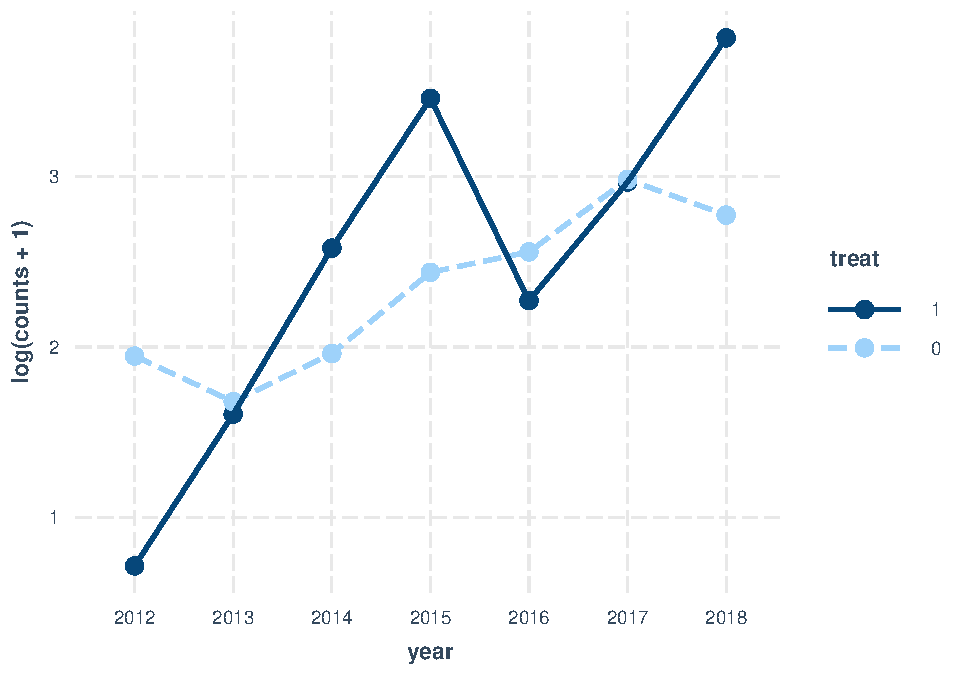
\includegraphics{hw1-lobstrs-eds241_files/figure-latex/unnamed-chunk-23-1.pdf}

\textbf{g.} Using \texttt{ggplot()} create a plot in same style as the
previous \texttt{interaction\ plot}, but displaying the original scale
of the outcome variable (lobster counts). This type of plot is commonly
used to show how the treatment effect changes across discrete time
points (i.e., panel data).

The plot should have\ldots{} - \texttt{year} on the x-axis -
\texttt{counts} on the y-axis - \texttt{mpa} as the grouping variable

\begin{Shaded}
\begin{Highlighting}[]
\CommentTok{\# Hint 1: Group counts by \textasciigrave{}year\textasciigrave{} and \textasciigrave{}mpa\textasciigrave{} and calculate the \textasciigrave{}mean\_count\textasciigrave{}}
\CommentTok{\# Hint 2: Convert variable \textasciigrave{}year\textasciigrave{} to a factor}

\NormalTok{plot\_counts }\OtherTok{\textless{}{-}}\NormalTok{ spiny\_counts }\SpecialCharTok{|\textgreater{}} 
    \FunctionTok{group\_by}\NormalTok{(year, mpa) }\SpecialCharTok{|\textgreater{}} 
    \FunctionTok{summarize}\NormalTok{(}\AttributeTok{mean\_counts =} \FunctionTok{mean}\NormalTok{(counts)) }\SpecialCharTok{|\textgreater{}} 
    \FunctionTok{mutate}\NormalTok{(}\AttributeTok{year =} \FunctionTok{as.factor}\NormalTok{(year)) }\SpecialCharTok{|\textgreater{}} 
    \FunctionTok{ggplot}\NormalTok{(}\FunctionTok{aes}\NormalTok{(}\AttributeTok{x =}\NormalTok{ year, }\AttributeTok{y =}\NormalTok{ mean\_counts, }\AttributeTok{color =}\NormalTok{ mpa)) }\SpecialCharTok{+}
    \FunctionTok{geom\_point}\NormalTok{() }\SpecialCharTok{+}
    \FunctionTok{geom\_line}\NormalTok{(}\FunctionTok{aes}\NormalTok{(}\AttributeTok{group =}\NormalTok{ mpa)) }\SpecialCharTok{+}
    \FunctionTok{labs}\NormalTok{(}
        \AttributeTok{title =} \StringTok{"Treatment Effect (MPA) Changes in Lobster Counts from 2012 to 2018"}\NormalTok{,}
        \AttributeTok{x =} \StringTok{"Year"}\NormalTok{,}
        \AttributeTok{y =} \StringTok{"Mean Lobster Counts"}
\NormalTok{    ) }\SpecialCharTok{+}
    \FunctionTok{scale\_color\_manual}\NormalTok{(}\AttributeTok{values =} \FunctionTok{c}\NormalTok{(}\StringTok{"navy"}\NormalTok{, }\StringTok{"lightblue3"}\NormalTok{ ),}
                       \AttributeTok{labels =} \FunctionTok{c}\NormalTok{(}\StringTok{"MPA"}\NormalTok{, }\StringTok{"Non{-}MPA"}\NormalTok{)) }\SpecialCharTok{+}
    \FunctionTok{scale\_linetype\_manual}\NormalTok{(}\AttributeTok{values =} \FunctionTok{c}\NormalTok{(}\StringTok{"solid"}\NormalTok{, }\StringTok{"longdash"}\NormalTok{))}

\FunctionTok{print}\NormalTok{(plot\_counts)}
\end{Highlighting}
\end{Shaded}

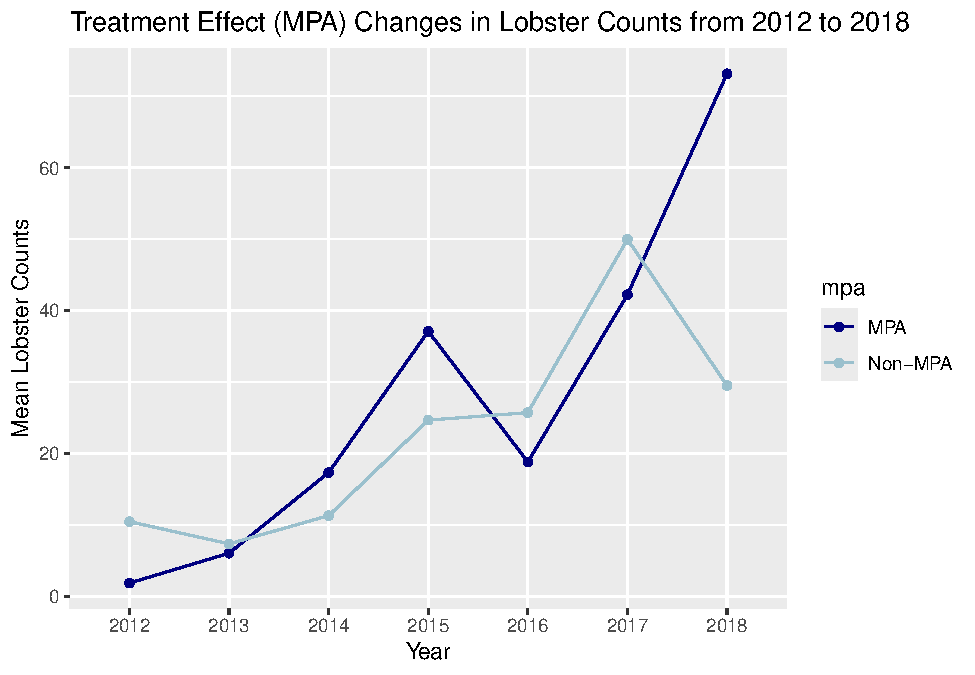
\includegraphics{hw1-lobstrs-eds241_files/figure-latex/unnamed-chunk-24-1.pdf}

\begin{center}\rule{0.5\linewidth}{0.5pt}\end{center}

Step 8: Reconsider causal identification assumptions

\begin{enumerate}
\def\labelenumi{\alph{enumi}.}
\tightlist
\item
  Discuss whether you think \texttt{spillover\ effects} are likely in
  this research context (see Glossary of terms;
  \url{https://docs.google.com/document/d/1RIudsVcYhWGpqC-Uftk9UTz3PIq6stVyEpT44EPNgpE/edit?usp=sharing})
\end{enumerate}

I think that there is likely at least some spillover in this research
context. The sites are all fairly close together (both MPA and non-MPA),
meaning that an increase in lobsters at an MPA site may have an effect
on the non-MPA sites, it could be as simple as lobsters moving from one
site to another.

\begin{enumerate}
\def\labelenumi{\alph{enumi}.}
\setcounter{enumi}{1}
\tightlist
\item
  Explain why spillover is an issue for the identification of causal
  effects
\end{enumerate}

Spillover is an issue for identifying causal effects because it would
mean that the treatment and control groups are not independent. The
treatment is also somehow affecting the control.

\begin{enumerate}
\def\labelenumi{\alph{enumi}.}
\setcounter{enumi}{2}
\tightlist
\item
  How does spillover relate to impact in this research setting?
\end{enumerate}

Spillover relates to impact because we can't trust that our counts at
our sites are independent of each other. The rise in counts in non-MPA
sites could be due to the MPA sites being nearby. We can't be sure of
the true impact of MPA sites.

\begin{enumerate}
\def\labelenumi{\alph{enumi}.}
\setcounter{enumi}{3}
\item
  Discuss the following causal inference assumptions in the context of
  the MPA treatment effect estimator. Evaluate if each of the assumption
  are reasonable:

  \begin{enumerate}
  \def\labelenumii{\arabic{enumii})}
  \tightlist
  \item
    SUTVA: Stable Unit Treatment Value assumption
  \item
    Excludability assumption
  \end{enumerate}
\end{enumerate}

SUTVA is not a reasonable assumption because we can assume there is a
spillover effect. The Stable Unit Treatment Value assumes that the
control and treatment groups are unaffected by each other. Because there
is spillover, it violates the key assumption in the SUTVA that there is
no interference of effect on MPAs on non-MPAs.

The Excludability assumption is that the treatment influences the
lobster counts at MPA sites and that the treatment (the MPA regulations)
are the only things influencing the treatment sites. This is not a
reasonable assumption in our research because if there is a spillover
effect we can't be sure that the treatment is actually influencing
lobster count differences between sites.

\begin{center}\rule{0.5\linewidth}{0.5pt}\end{center}

\section{EXTRA CREDIT}\label{extra-credit}

\begin{quote}
Use the recent lobster abundance data with observations collected up
until 2024 (\texttt{lobster\_sbchannel\_24.csv}) to run an analysis
evaluating the effect of MPA status on lobster counts using the same
focal variables.
\end{quote}

\begin{enumerate}
\def\labelenumi{\alph{enumi}.}
\tightlist
\item
  Create a new script for the analysis on the updated data
\end{enumerate}

\begin{Shaded}
\begin{Highlighting}[]
\NormalTok{recent\_lobster }\OtherTok{\textless{}{-}} \FunctionTok{read\_csv}\NormalTok{(}\FunctionTok{here}\NormalTok{(}\StringTok{"data"}\NormalTok{, }\StringTok{"lobster\_sbchannel\_24.csv"}\NormalTok{)) }\SpecialCharTok{|\textgreater{}} 
    \FunctionTok{clean\_names}\NormalTok{() }\SpecialCharTok{|\textgreater{}} 
\NormalTok{    naniar}\SpecialCharTok{::}\FunctionTok{replace\_with\_na}\NormalTok{(}\AttributeTok{replace =} \FunctionTok{list}\NormalTok{(}\AttributeTok{size\_mm =} \SpecialCharTok{{-}}\DecValTok{99999}\NormalTok{))}
\end{Highlighting}
\end{Shaded}

\begin{Shaded}
\begin{Highlighting}[]
\NormalTok{recent\_lobster\_clean }\OtherTok{\textless{}{-}}\NormalTok{ recent\_lobster }\SpecialCharTok{|\textgreater{}}    
    \FunctionTok{mutate}\NormalTok{(}\AttributeTok{reef =} \FunctionTok{factor}\NormalTok{(site, }\AttributeTok{order =} \ConstantTok{TRUE}\NormalTok{, }\AttributeTok{levels =} \FunctionTok{c}\NormalTok{(}\StringTok{"AQUE"}\NormalTok{, }\StringTok{"CARP"}\NormalTok{, }\StringTok{"MOHK"}\NormalTok{, }\StringTok{"IVEE"}\NormalTok{, }\StringTok{"NAPL"}\NormalTok{), }\AttributeTok{labels =} \FunctionTok{c}\NormalTok{(}\StringTok{"Arroyo Quemado"}\NormalTok{, }\StringTok{"Carpenteria"}\NormalTok{, }\StringTok{"Mohawk"}\NormalTok{, }\StringTok{"Isla Vista"}\NormalTok{,  }\StringTok{"Naples"}\NormalTok{))) }
\end{Highlighting}
\end{Shaded}

\begin{Shaded}
\begin{Highlighting}[]
\NormalTok{recent\_counts }\OtherTok{\textless{}{-}}\NormalTok{ recent\_lobster\_clean }\SpecialCharTok{|\textgreater{}} 
    \FunctionTok{group\_by}\NormalTok{(site, year, transect) }\SpecialCharTok{|\textgreater{}} 
    \FunctionTok{summarize}\NormalTok{(}\AttributeTok{counts =} \FunctionTok{sum}\NormalTok{(count, }\AttributeTok{na.rm =} \ConstantTok{TRUE}\NormalTok{),}
              \AttributeTok{mean\_size =} \FunctionTok{mean}\NormalTok{(size\_mm, }\AttributeTok{na.rm =} \ConstantTok{TRUE}\NormalTok{)) }\SpecialCharTok{|\textgreater{}} 
    \FunctionTok{mutate}\NormalTok{(}\AttributeTok{mpa =} \FunctionTok{case\_when}\NormalTok{(}
\NormalTok{        site }\SpecialCharTok{\%in\%} \FunctionTok{c}\NormalTok{(}\StringTok{"IVEE"}\NormalTok{, }\StringTok{"NAPL"}\NormalTok{) }\SpecialCharTok{\textasciitilde{}} \StringTok{"MPA"}\NormalTok{,}
\NormalTok{        site }\SpecialCharTok{\%in\%} \FunctionTok{c}\NormalTok{(}\StringTok{"AQUE"}\NormalTok{, }\StringTok{"CARP"}\NormalTok{, }\StringTok{"MOHK"}\NormalTok{) }\SpecialCharTok{\textasciitilde{}} \StringTok{"non\_MPA"}
\NormalTok{    ), }\AttributeTok{treat =} \FunctionTok{case\_when}\NormalTok{(mpa }\SpecialCharTok{==} \StringTok{"MPA"} \SpecialCharTok{\textasciitilde{}} \DecValTok{1}\NormalTok{,}
\NormalTok{                        mpa }\SpecialCharTok{==} \StringTok{"non\_MPA"} \SpecialCharTok{\textasciitilde{}} \DecValTok{0}\NormalTok{))}
\end{Highlighting}
\end{Shaded}

\begin{Shaded}
\begin{Highlighting}[]
\CommentTok{\# plot 1: density ridge plot}
\NormalTok{plot1 }\OtherTok{\textless{}{-}}\NormalTok{ recent\_counts }\SpecialCharTok{|\textgreater{}} 
    \FunctionTok{ggplot}\NormalTok{(}\FunctionTok{aes}\NormalTok{(}\AttributeTok{x =}\NormalTok{ counts, }\AttributeTok{y =}\NormalTok{ site)) }\SpecialCharTok{+}
    \FunctionTok{geom\_density\_ridges2}\NormalTok{(}\AttributeTok{quantile\_lines =} \ConstantTok{TRUE}\NormalTok{,}
                         \AttributeTok{alpha =} \FloatTok{0.3}\NormalTok{,}
                         \AttributeTok{fill =} \StringTok{"blue3"}\NormalTok{,}
                         \AttributeTok{color =} \StringTok{"navy"}\NormalTok{) }\SpecialCharTok{+}
    \FunctionTok{labs}\NormalTok{(}
        \AttributeTok{title =} \StringTok{"Density Plot of Spiny Lobster Counts by Reef Site"}\NormalTok{,}
        \AttributeTok{subtitle =} \StringTok{"(including quartiles as descriptive statistic)"}\NormalTok{,}
        \AttributeTok{x =} \StringTok{"Spiny Lobster Counts"}\NormalTok{,}
        \AttributeTok{y =} \StringTok{"Density"}\NormalTok{) }\SpecialCharTok{+}
    \FunctionTok{theme\_bw}\NormalTok{()}

\FunctionTok{print}\NormalTok{(plot1)}
\end{Highlighting}
\end{Shaded}

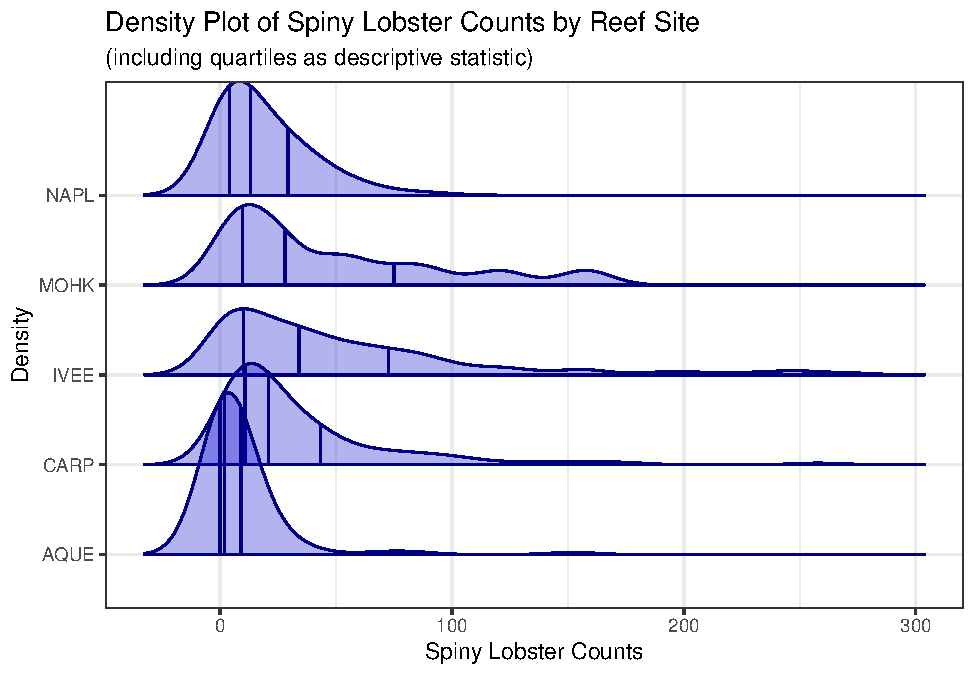
\includegraphics{hw1-lobstrs-eds241_files/figure-latex/unnamed-chunk-28-1.pdf}

\begin{Shaded}
\begin{Highlighting}[]
\CommentTok{\# plot 2: beeswarm (with boxplot)}

\NormalTok{plot2 }\OtherTok{\textless{}{-}} \FunctionTok{ggplot}\NormalTok{(recent\_counts, }\FunctionTok{aes}\NormalTok{(}\AttributeTok{x =}\NormalTok{ mpa, }\AttributeTok{y =}\NormalTok{ counts)) }\SpecialCharTok{+}
    \FunctionTok{geom\_boxplot}\NormalTok{(}\AttributeTok{outlier.shape =} \ConstantTok{NA}\NormalTok{) }\SpecialCharTok{+}
\NormalTok{    ggbeeswarm}\SpecialCharTok{::}\FunctionTok{geom\_beeswarm}\NormalTok{(}\AttributeTok{size =} \DecValTok{1}\NormalTok{, }\AttributeTok{alpha =}\NormalTok{ .}\DecValTok{4}\NormalTok{, }\AttributeTok{color =} \StringTok{"orange4"}\NormalTok{) }\SpecialCharTok{+}
    \FunctionTok{scale\_y\_continuous}\NormalTok{(}\AttributeTok{limits =} \FunctionTok{quantile}\NormalTok{(spiny\_counts}\SpecialCharTok{$}\NormalTok{counts, }\FunctionTok{c}\NormalTok{(}\FloatTok{0.1}\NormalTok{, }\FloatTok{0.9}\NormalTok{))) }\SpecialCharTok{+}
    \FunctionTok{theme\_bw}\NormalTok{() }\SpecialCharTok{+}
    \FunctionTok{labs}\NormalTok{(}
        \AttributeTok{title =} \StringTok{"Boxplot with Beeswarm Overlay of Spiny Lobster Counts by MPA Status"}\NormalTok{,}
        \AttributeTok{x =} \StringTok{"MPA Status"}\NormalTok{,}
        \AttributeTok{y =} \StringTok{"Lobster Counts"}\NormalTok{) }
\FunctionTok{print}\NormalTok{(plot2)   }
\end{Highlighting}
\end{Shaded}

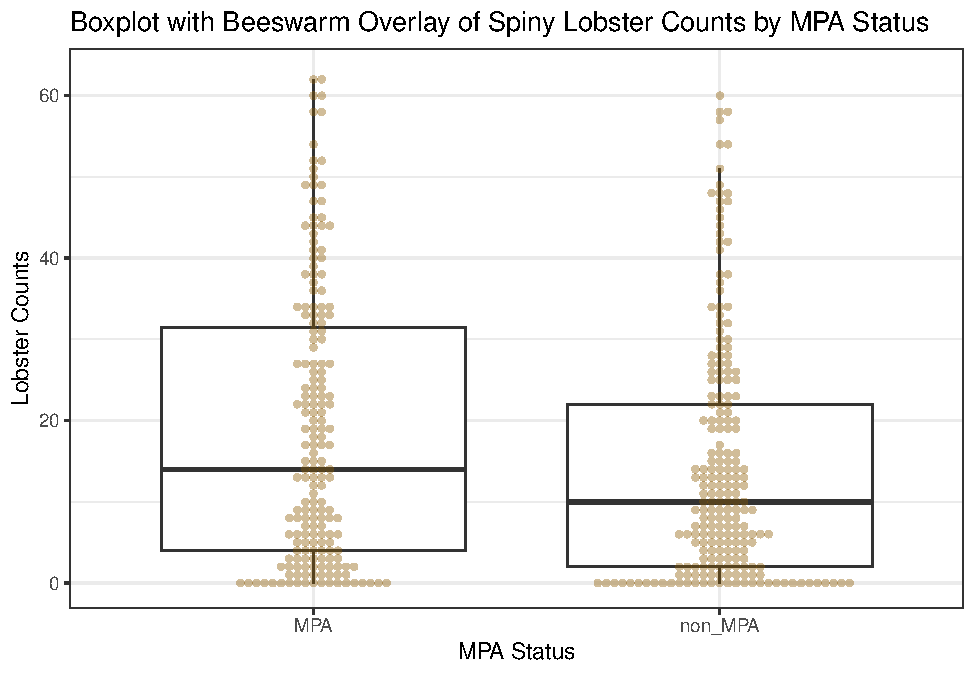
\includegraphics{hw1-lobstrs-eds241_files/figure-latex/unnamed-chunk-28-2.pdf}

\begin{Shaded}
\begin{Highlighting}[]
\CommentTok{\# plot 3: violin plot}

\NormalTok{plot3 }\OtherTok{\textless{}{-}} \FunctionTok{ggplot}\NormalTok{(recent\_counts, }\FunctionTok{aes}\NormalTok{(}\AttributeTok{x =} \FunctionTok{as.factor}\NormalTok{(year), }\AttributeTok{y =}\NormalTok{ counts)) }\SpecialCharTok{+}
    \FunctionTok{geom\_violin}\NormalTok{(}\AttributeTok{color =} \StringTok{"green4"}\NormalTok{, }\AttributeTok{fill =} \StringTok{"green3"}\NormalTok{) }\SpecialCharTok{+}
    \FunctionTok{stat\_summary}\NormalTok{(}\AttributeTok{fun.y=}\NormalTok{median, }\AttributeTok{geom=}\StringTok{"crossbar"}\NormalTok{, }\AttributeTok{size=}\NormalTok{.}\DecValTok{3}\NormalTok{, }\AttributeTok{color=}\StringTok{"black"}\NormalTok{) }\SpecialCharTok{+}
    \FunctionTok{scale\_y\_continuous}\NormalTok{(}\AttributeTok{limits =} \FunctionTok{quantile}\NormalTok{(spiny\_counts}\SpecialCharTok{$}\NormalTok{counts, }\FunctionTok{c}\NormalTok{(}\FloatTok{0.1}\NormalTok{, }\FloatTok{0.9}\NormalTok{))) }\SpecialCharTok{+}
    \FunctionTok{theme\_bw}\NormalTok{() }\SpecialCharTok{+}
    \FunctionTok{labs}\NormalTok{(}
        \AttributeTok{title =} \StringTok{"Violin Plot of Spiny Lobster Counts by Year (2012{-}2024)"}\NormalTok{,}
        \AttributeTok{subtitle =} \StringTok{"(including medians as the descriptive statistic)"}\NormalTok{,}
        \AttributeTok{x =} \StringTok{"Year"}\NormalTok{,}
        \AttributeTok{y =} \StringTok{"Spiny Lobster Counts"}\NormalTok{)}

\FunctionTok{print}\NormalTok{(plot3)}
\end{Highlighting}
\end{Shaded}

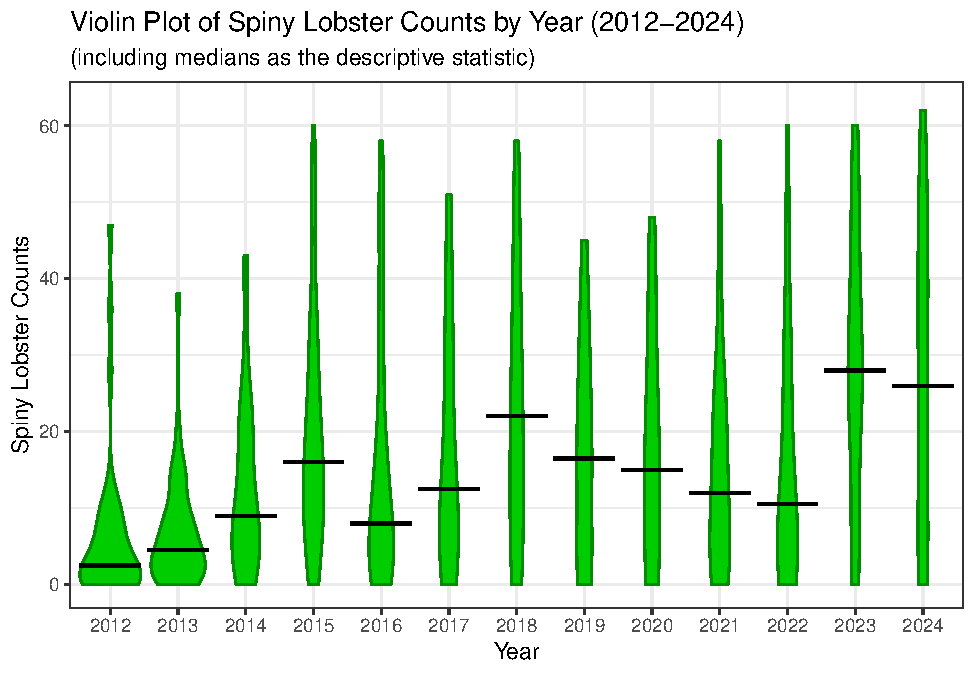
\includegraphics{hw1-lobstrs-eds241_files/figure-latex/unnamed-chunk-28-3.pdf}

\begin{Shaded}
\begin{Highlighting}[]
\CommentTok{\# plot 4: jitter plot}

\NormalTok{plot4 }\OtherTok{\textless{}{-}} \FunctionTok{ggplot}\NormalTok{(recent\_counts, }\FunctionTok{aes}\NormalTok{(}\AttributeTok{x =}\NormalTok{ year, }\AttributeTok{y =}\NormalTok{ mean\_size)) }\SpecialCharTok{+}
    \FunctionTok{geom\_jitter}\NormalTok{(}\AttributeTok{color =} \StringTok{"darkred"}\NormalTok{, }\AttributeTok{size =} \FloatTok{1.2}\NormalTok{) }\SpecialCharTok{+}
    \FunctionTok{theme\_bw}\NormalTok{() }\SpecialCharTok{+}
    \FunctionTok{labs}\NormalTok{(}
        \AttributeTok{title =} \StringTok{"Jitter Plot of Spiny Lobster Average Size by Year (2012{-}2024)"}\NormalTok{,}
        \AttributeTok{x =} \StringTok{"Year"}\NormalTok{,}
        \AttributeTok{y =} \StringTok{"Average Lobster Size"}\NormalTok{) }\SpecialCharTok{+}
     \FunctionTok{scale\_x\_continuous}\NormalTok{(}\AttributeTok{limits=}\FunctionTok{c}\NormalTok{(}\DecValTok{2012}\NormalTok{, }\DecValTok{2018}\NormalTok{), }\AttributeTok{expand =} \FunctionTok{c}\NormalTok{(}\DecValTok{0}\NormalTok{,}\ConstantTok{NA}\NormalTok{))}
    

\FunctionTok{print}\NormalTok{(plot4)}
\end{Highlighting}
\end{Shaded}

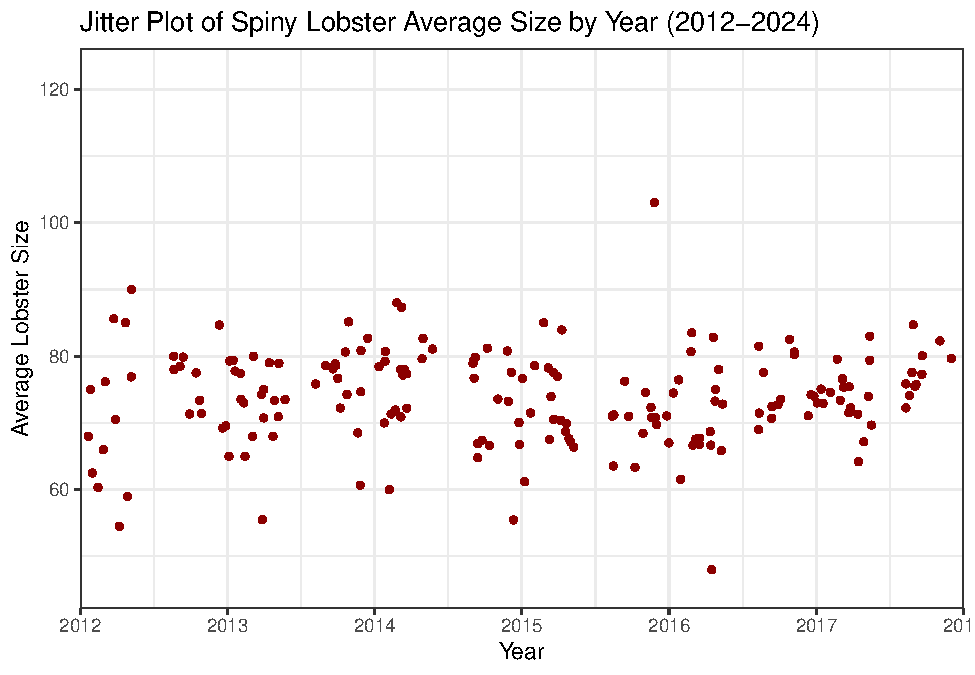
\includegraphics{hw1-lobstrs-eds241_files/figure-latex/unnamed-chunk-28-4.pdf}

\begin{Shaded}
\begin{Highlighting}[]
\NormalTok{recent\_counts }\SpecialCharTok{|\textgreater{}} 
\NormalTok{    dplyr}\SpecialCharTok{::}\FunctionTok{select}\NormalTok{(counts, mean\_size, mpa) }\SpecialCharTok{|\textgreater{}}
    \FunctionTok{tbl\_summary}\NormalTok{(}\AttributeTok{by =}\NormalTok{ mpa,}
                \AttributeTok{statistic =} \FunctionTok{list}\NormalTok{(}\FunctionTok{all\_continuous}\NormalTok{() }\SpecialCharTok{\textasciitilde{}} \StringTok{"\{mean\}"}\NormalTok{)) }\SpecialCharTok{|\textgreater{}}
    \FunctionTok{modify\_caption}\NormalTok{(}\StringTok{"**Comparing the mean counts and mean sizes of California Spiny Lobsters at MPA and non{-}MPA sites**"}\NormalTok{)}
\end{Highlighting}
\end{Shaded}

\begin{table}[!t]
\caption{\label{tab:unnamed-chunk-29}\textbf{Comparing the mean counts and mean sizes of California Spiny Lobsters at MPA and non-MPA sites}} 
\fontsize{12.0pt}{14.4pt}\selectfont
\begin{tabular*}{\linewidth}{@{\extracolsep{\fill}}lcc}
\toprule
\textbf{Characteristic} & \textbf{MPA}  N = 220\textsuperscript{\textit{1}} & \textbf{non\_MPA}  N = 246\textsuperscript{\textit{1}} \\ 
\midrule\addlinespace[2.5pt]
site &  &  \\ 
    AQUE & 0 (0\%) & 91 (37\%) \\ 
    CARP & 0 (0\%) & 116 (47\%) \\ 
    IVEE & 104 (47\%) & 0 (0\%) \\ 
    MOHK & 0 (0\%) & 39 (16\%) \\ 
    NAPL & 116 (53\%) & 0 (0\%) \\ 
year & 2,018.0 & 2,018.0 \\ 
counts & 35 & 27 \\ 
mean\_size & 80 & 74 \\ 
    Unknown & 19 & 32 \\ 
\bottomrule
\end{tabular*}
\begin{minipage}{\linewidth}
\textsuperscript{\textit{1}}n (\%); Mean\\
\end{minipage}
\end{table}

\begin{enumerate}
\def\labelenumi{\alph{enumi}.}
\setcounter{enumi}{1}
\tightlist
\item
  Run at least 3 regression models \& assess model diagnostics
\end{enumerate}

\begin{Shaded}
\begin{Highlighting}[]
\NormalTok{m1\_ols\_recent }\OtherTok{\textless{}{-}} \FunctionTok{lm}\NormalTok{(counts }\SpecialCharTok{\textasciitilde{}}\NormalTok{ treat, }\AttributeTok{data =}\NormalTok{ recent\_counts)}

\FunctionTok{summ}\NormalTok{(m1\_ols\_recent, }\AttributeTok{model.fit =} \ConstantTok{FALSE}\NormalTok{) }
\end{Highlighting}
\end{Shaded}

\begin{table}[!h]
\centering
\begin{tabular}{lr}
\toprule
\cellcolor{gray!10}{Observations} & \cellcolor{gray!10}{466}\\
Dependent variable & counts\\
\cellcolor{gray!10}{Type} & \cellcolor{gray!10}{OLS linear regression}\\
\bottomrule
\end{tabular}
\end{table}  \begin{table}[!h]
\centering
\begin{threeparttable}
\begin{tabular}{lrrrr}
\toprule
  & Est. & S.E. & t val. & p\\
\midrule
\cellcolor{gray!10}{(Intercept)} & \cellcolor{gray!10}{27.27} & \cellcolor{gray!10}{2.69} & \cellcolor{gray!10}{10.15} & \cellcolor{gray!10}{0.00}\\
treat & 7.72 & 3.91 & 1.97 & 0.05\\
\bottomrule
\end{tabular}
\begin{tablenotes}
\item Standard errors: OLS
\end{tablenotes}
\end{threeparttable}
\end{table}

\begin{Shaded}
\begin{Highlighting}[]
\FunctionTok{print}\NormalTok{(}\FunctionTok{check\_model}\NormalTok{(m1\_ols\_recent,  }\AttributeTok{check =} \StringTok{"qq"}\NormalTok{ ))}
\end{Highlighting}
\end{Shaded}

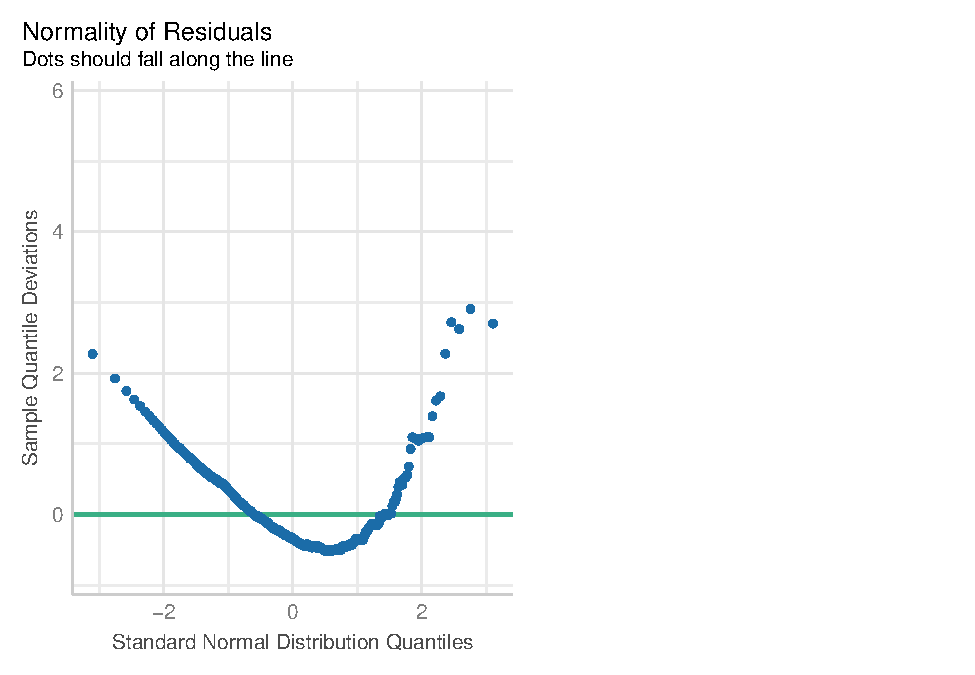
\includegraphics{hw1-lobstrs-eds241_files/figure-latex/unnamed-chunk-31-1.pdf}

\begin{Shaded}
\begin{Highlighting}[]
\FunctionTok{print}\NormalTok{(}\FunctionTok{check\_model}\NormalTok{(m1\_ols\_recent, }\AttributeTok{check =} \StringTok{"normality"}\NormalTok{))}
\end{Highlighting}
\end{Shaded}

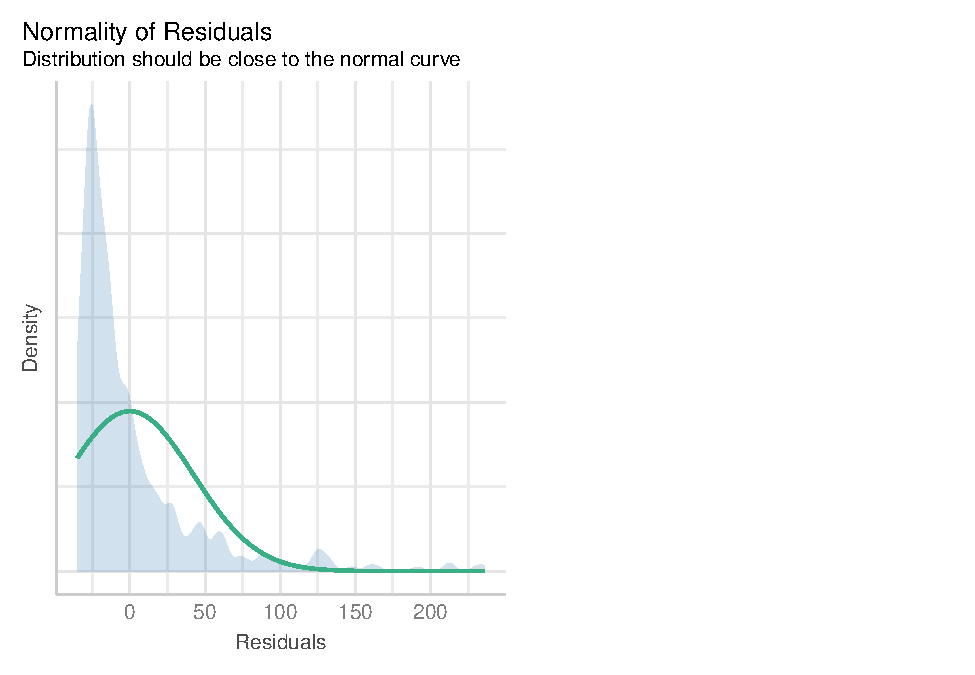
\includegraphics{hw1-lobstrs-eds241_files/figure-latex/unnamed-chunk-32-1.pdf}

\begin{Shaded}
\begin{Highlighting}[]
\FunctionTok{print}\NormalTok{(}\FunctionTok{check\_model}\NormalTok{(m1\_ols\_recent, }\AttributeTok{check =} \StringTok{"homogeneity"}\NormalTok{))}
\end{Highlighting}
\end{Shaded}

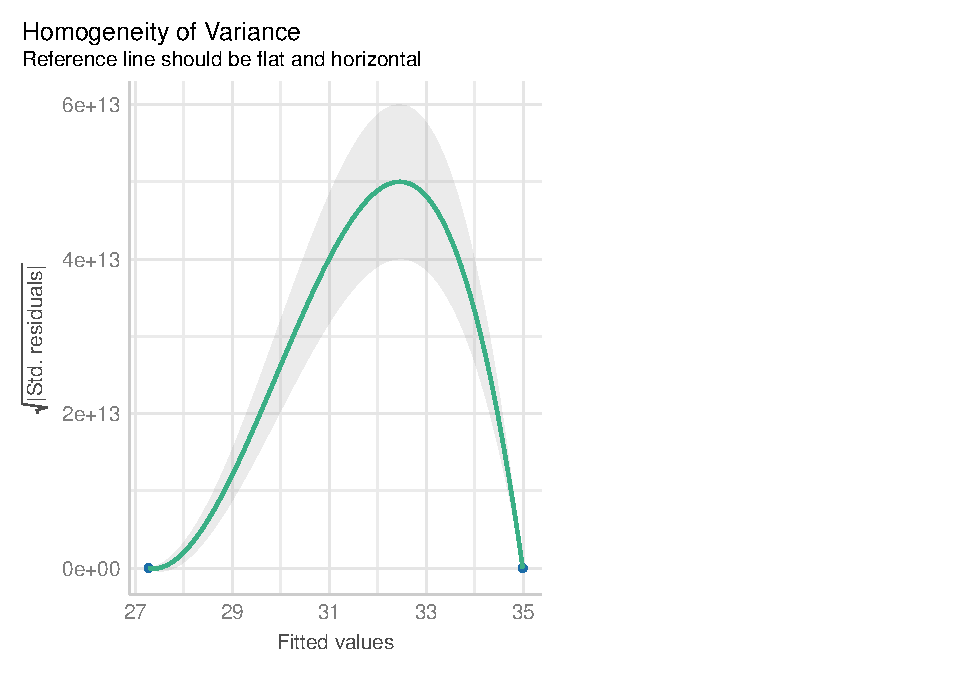
\includegraphics{hw1-lobstrs-eds241_files/figure-latex/unnamed-chunk-33-1.pdf}

\begin{Shaded}
\begin{Highlighting}[]
\FunctionTok{print}\NormalTok{(}\FunctionTok{check\_model}\NormalTok{(m1\_ols\_recent, }\AttributeTok{check =} \StringTok{"pp\_check"}\NormalTok{))}
\end{Highlighting}
\end{Shaded}

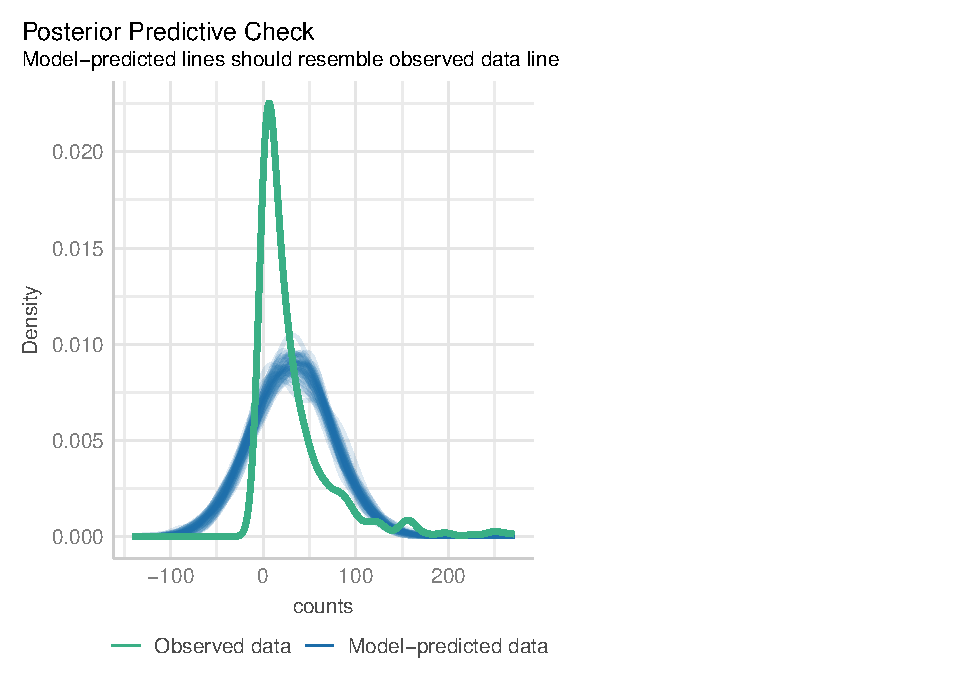
\includegraphics{hw1-lobstrs-eds241_files/figure-latex/unnamed-chunk-34-1.pdf}

\begin{Shaded}
\begin{Highlighting}[]
\NormalTok{m2\_pois\_recent }\OtherTok{\textless{}{-}} \FunctionTok{glm}\NormalTok{(counts }\SpecialCharTok{\textasciitilde{}}\NormalTok{ treat,}
\NormalTok{               recent\_counts,}
               \AttributeTok{family =} \FunctionTok{poisson}\NormalTok{(}\AttributeTok{link =} \StringTok{"log"}\NormalTok{))}

\FunctionTok{summ}\NormalTok{(m2\_pois\_recent)}
\end{Highlighting}
\end{Shaded}

\begin{table}[!h]
\centering
\begin{tabular}{lr}
\toprule
\cellcolor{gray!10}{Observations} & \cellcolor{gray!10}{466}\\
Dependent variable & counts\\
\cellcolor{gray!10}{Type} & \cellcolor{gray!10}{Generalized linear model}\\
Family & poisson\\
\cellcolor{gray!10}{Link} & \cellcolor{gray!10}{log}\\
\bottomrule
\end{tabular}
\end{table} \begin{table}[!h]
\centering
\begin{tabular}{lr}
\toprule
\cellcolor{gray!10}{$\chi^2$(1)} & \cellcolor{gray!10}{223.34}\\
p & 0.00\\
\cellcolor{gray!10}{Pseudo-R² (Cragg-Uhler)} & \cellcolor{gray!10}{0.38}\\
Pseudo-R² (McFadden) & 0.01\\
\cellcolor{gray!10}{AIC} & \cellcolor{gray!10}{21530.09}\\
\addlinespace
BIC & 21538.38\\
\bottomrule
\end{tabular}
\end{table} \begin{table}[!h]
\centering
\begin{threeparttable}
\begin{tabular}{lrrrr}
\toprule
  & Est. & S.E. & z val. & p\\
\midrule
\cellcolor{gray!10}{(Intercept)} & \cellcolor{gray!10}{3.31} & \cellcolor{gray!10}{0.01} & \cellcolor{gray!10}{270.75} & \cellcolor{gray!10}{0.00}\\
treat & 0.25 & 0.02 & 14.92 & 0.00\\
\bottomrule
\end{tabular}
\begin{tablenotes}
\item Standard errors: MLE
\end{tablenotes}
\end{threeparttable}
\end{table}

\begin{Shaded}
\begin{Highlighting}[]
\FunctionTok{print}\NormalTok{(}\FunctionTok{exp}\NormalTok{(.}\DecValTok{25}\NormalTok{) }\SpecialCharTok{{-}} \DecValTok{1}\NormalTok{)}
\end{Highlighting}
\end{Shaded}

\begin{verbatim}
## [1] 0.2840254
\end{verbatim}

\begin{Shaded}
\begin{Highlighting}[]
\FunctionTok{print}\NormalTok{(}\FunctionTok{check\_model}\NormalTok{(m2\_pois\_recent))}
\end{Highlighting}
\end{Shaded}

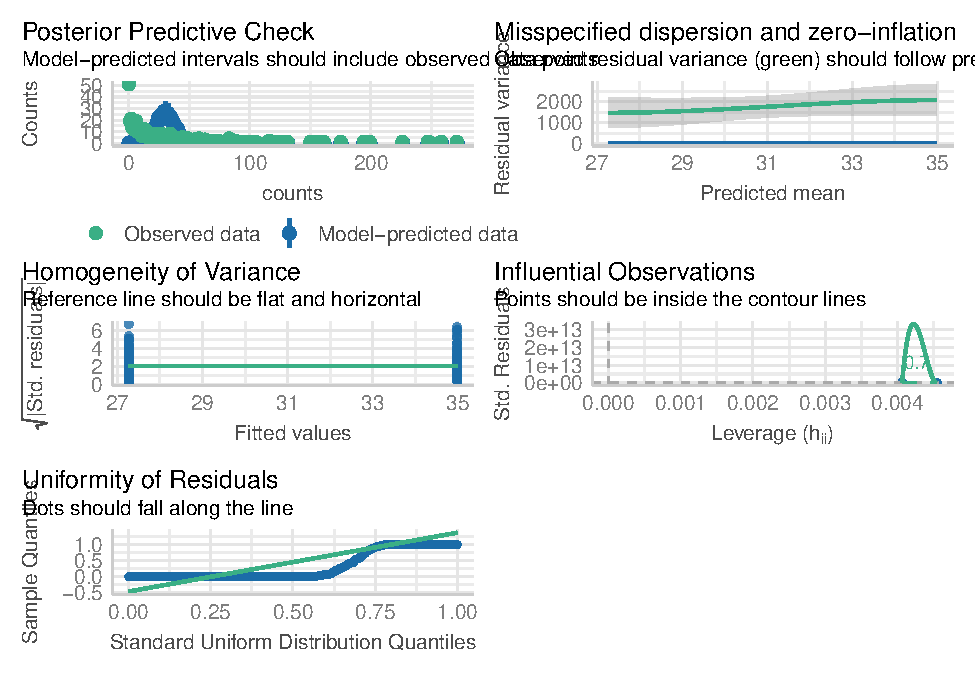
\includegraphics{hw1-lobstrs-eds241_files/figure-latex/unnamed-chunk-36-1.pdf}

\begin{Shaded}
\begin{Highlighting}[]
\FunctionTok{print}\NormalTok{(}\FunctionTok{check\_overdispersion}\NormalTok{(m2\_pois\_recent))}
\end{Highlighting}
\end{Shaded}

\begin{verbatim}
## # Overdispersion test
## 
##        dispersion ratio =    57.103
##   Pearson's Chi-Squared = 26496.023
##                 p-value =   < 0.001
\end{verbatim}

\begin{Shaded}
\begin{Highlighting}[]
\FunctionTok{print}\NormalTok{(}\FunctionTok{check\_zeroinflation}\NormalTok{(m2\_pois\_recent))}
\end{Highlighting}
\end{Shaded}

\begin{verbatim}
## # Check for zero-inflation
## 
##    Observed zeros: 51
##   Predicted zeros: 0
##             Ratio: 0.00
\end{verbatim}

\begin{Shaded}
\begin{Highlighting}[]
\NormalTok{m3\_nb\_recent }\OtherTok{\textless{}{-}}\NormalTok{ MASS}\SpecialCharTok{::}\FunctionTok{glm.nb}\NormalTok{(counts }\SpecialCharTok{\textasciitilde{}}\NormalTok{ treat,}
\NormalTok{               recent\_counts)}

\FunctionTok{summ}\NormalTok{(m3\_nb\_recent)}
\end{Highlighting}
\end{Shaded}

\begin{table}[!h]
\centering
\begin{tabular}{lr}
\toprule
\cellcolor{gray!10}{Observations} & \cellcolor{gray!10}{466}\\
Dependent variable & counts\\
\cellcolor{gray!10}{Type} & \cellcolor{gray!10}{Generalized linear model}\\
Family & Negative Binomial(0.5769)\\
\cellcolor{gray!10}{Link} & \cellcolor{gray!10}{log}\\
\bottomrule
\end{tabular}
\end{table} \begin{table}[!h]
\centering
\begin{tabular}{lr}
\toprule
\cellcolor{gray!10}{$\chi^2$(464)} & \cellcolor{gray!10}{4.08}\\
p & 0.04\\
\cellcolor{gray!10}{Pseudo-R² (Cragg-Uhler)} & \cellcolor{gray!10}{0.01}\\
Pseudo-R² (McFadden) & 0.00\\
\cellcolor{gray!10}{AIC} & \cellcolor{gray!10}{4058.04}\\
\addlinespace
BIC & 4070.48\\
\bottomrule
\end{tabular}
\end{table} \begin{table}[!h]
\centering
\begin{threeparttable}
\begin{tabular}{lrrrr}
\toprule
  & Est. & S.E. & z val. & p\\
\midrule
\cellcolor{gray!10}{(Intercept)} & \cellcolor{gray!10}{3.31} & \cellcolor{gray!10}{0.08} & \cellcolor{gray!10}{38.97} & \cellcolor{gray!10}{0.00}\\
treat & 0.25 & 0.12 & 2.02 & 0.04\\
\bottomrule
\end{tabular}
\begin{tablenotes}
\item Standard errors: MLE
\end{tablenotes}
\end{threeparttable}
\end{table}

\begin{Shaded}
\begin{Highlighting}[]
\FunctionTok{print}\NormalTok{(}\FunctionTok{exp}\NormalTok{(.}\DecValTok{25}\NormalTok{) }\SpecialCharTok{{-}} \DecValTok{1}\NormalTok{)}
\end{Highlighting}
\end{Shaded}

\begin{verbatim}
## [1] 0.2840254
\end{verbatim}

\begin{Shaded}
\begin{Highlighting}[]
\FunctionTok{print}\NormalTok{(}\FunctionTok{check\_overdispersion}\NormalTok{(m3\_nb\_recent))}
\end{Highlighting}
\end{Shaded}

\begin{verbatim}
## # Overdispersion test
## 
##  dispersion ratio = 1.035
##           p-value = 0.808
\end{verbatim}

\begin{Shaded}
\begin{Highlighting}[]
\FunctionTok{print}\NormalTok{(}\FunctionTok{check\_zeroinflation}\NormalTok{(m3\_nb\_recent))}
\end{Highlighting}
\end{Shaded}

\begin{verbatim}
## # Check for zero-inflation
## 
##    Observed zeros: 51
##   Predicted zeros: 47
##             Ratio: 0.91
\end{verbatim}

\begin{Shaded}
\begin{Highlighting}[]
\FunctionTok{print}\NormalTok{(}\FunctionTok{check\_predictions}\NormalTok{(m3\_nb\_recent))}
\end{Highlighting}
\end{Shaded}

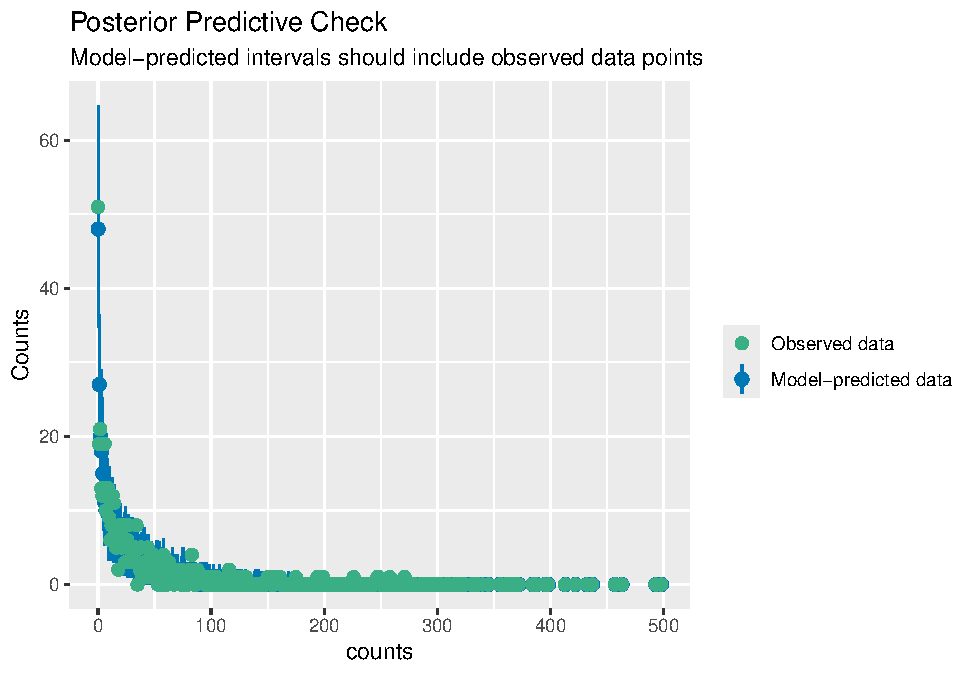
\includegraphics{hw1-lobstrs-eds241_files/figure-latex/unnamed-chunk-42-1.pdf}

\begin{Shaded}
\begin{Highlighting}[]
\FunctionTok{print}\NormalTok{(}\FunctionTok{check\_model}\NormalTok{(m3\_nb\_recent))}
\end{Highlighting}
\end{Shaded}

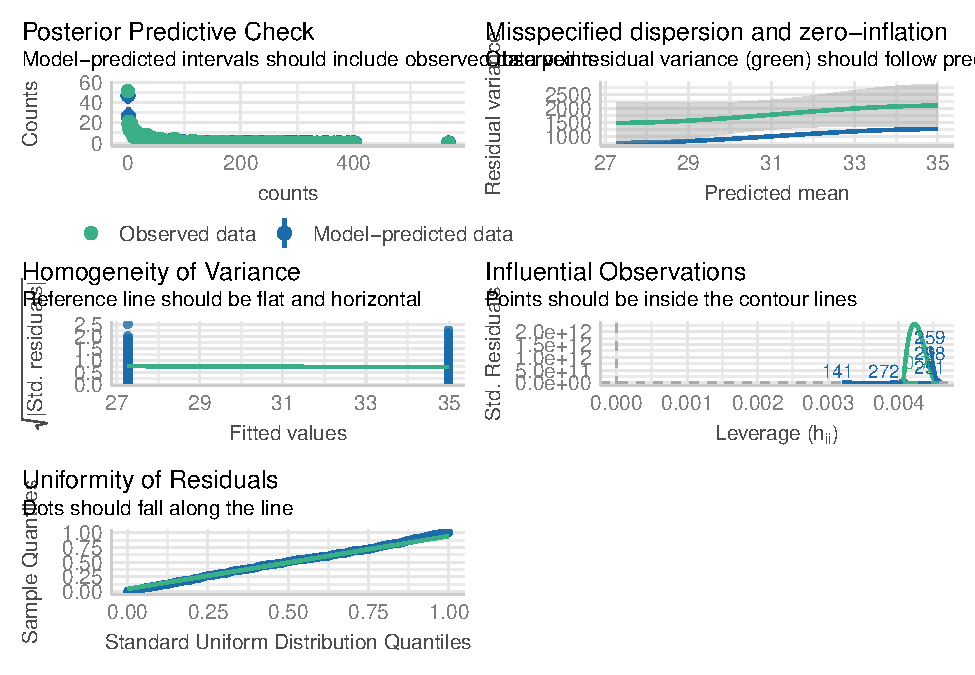
\includegraphics{hw1-lobstrs-eds241_files/figure-latex/unnamed-chunk-43-1.pdf}

\begin{Shaded}
\begin{Highlighting}[]
\FunctionTok{export\_summs}\NormalTok{(m1\_ols\_recent, m2\_pois\_recent, m3\_nb\_recent,}
             \AttributeTok{model.names =} \FunctionTok{c}\NormalTok{(}\StringTok{"OLS"}\NormalTok{,}\StringTok{"Poisson"}\NormalTok{, }\StringTok{"NB"}\NormalTok{))}
\end{Highlighting}
\end{Shaded}

 
  \providecommand{\huxb}[2]{\arrayrulecolor[RGB]{#1}\global\arrayrulewidth=#2pt}
  \providecommand{\huxvb}[2]{\color[RGB]{#1}\vrule width #2pt}
  \providecommand{\huxtpad}[1]{\rule{0pt}{#1}}
  \providecommand{\huxbpad}[1]{\rule[-#1]{0pt}{#1}}

\begin{table}[ht]
\begin{centerbox}
\begin{threeparttable}
 \setlength{\tabcolsep}{0pt}
\begin{tabular}{l l l l}


\hhline{>{\huxb{0, 0, 0}{0.8}}->{\huxb{0, 0, 0}{0.8}}->{\huxb{0, 0, 0}{0.8}}->{\huxb{0, 0, 0}{0.8}}-}
\arrayrulecolor{black}

\multicolumn{1}{!{\huxvb{0, 0, 0}{0}}c!{\huxvb{0, 0, 0}{0}}}{\huxtpad{6pt + 1em}\centering \hspace{6pt}  \hspace{6pt}\huxbpad{6pt}} &
\multicolumn{1}{c!{\huxvb{0, 0, 0}{0}}}{\huxtpad{6pt + 1em}\centering \hspace{6pt} OLS \hspace{6pt}\huxbpad{6pt}} &
\multicolumn{1}{c!{\huxvb{0, 0, 0}{0}}}{\huxtpad{6pt + 1em}\centering \hspace{6pt} Poisson \hspace{6pt}\huxbpad{6pt}} &
\multicolumn{1}{c!{\huxvb{0, 0, 0}{0}}}{\huxtpad{6pt + 1em}\centering \hspace{6pt} NB \hspace{6pt}\huxbpad{6pt}} \tabularnewline[-0.5pt]


\hhline{>{\huxb{255, 255, 255}{0.4}}->{\huxb{0, 0, 0}{0.4}}->{\huxb{0, 0, 0}{0.4}}->{\huxb{0, 0, 0}{0.4}}-}
\arrayrulecolor{black}

\multicolumn{1}{!{\huxvb{0, 0, 0}{0}}l!{\huxvb{0, 0, 0}{0}}}{\huxtpad{6pt + 1em}\raggedright \hspace{6pt} (Intercept) \hspace{6pt}\huxbpad{6pt}} &
\multicolumn{1}{r!{\huxvb{0, 0, 0}{0}}}{\huxtpad{6pt + 1em}\raggedleft \hspace{6pt} 27.27 *** \hspace{6pt}\huxbpad{6pt}} &
\multicolumn{1}{r!{\huxvb{0, 0, 0}{0}}}{\huxtpad{6pt + 1em}\raggedleft \hspace{6pt} 3.31 *** \hspace{6pt}\huxbpad{6pt}} &
\multicolumn{1}{r!{\huxvb{0, 0, 0}{0}}}{\huxtpad{6pt + 1em}\raggedleft \hspace{6pt} 3.31 *** \hspace{6pt}\huxbpad{6pt}} \tabularnewline[-0.5pt]


\hhline{}
\arrayrulecolor{black}

\multicolumn{1}{!{\huxvb{0, 0, 0}{0}}l!{\huxvb{0, 0, 0}{0}}}{\huxtpad{6pt + 1em}\raggedright \hspace{6pt}  \hspace{6pt}\huxbpad{6pt}} &
\multicolumn{1}{r!{\huxvb{0, 0, 0}{0}}}{\huxtpad{6pt + 1em}\raggedleft \hspace{6pt} (2.69)\hphantom{0}\hphantom{0}\hphantom{0} \hspace{6pt}\huxbpad{6pt}} &
\multicolumn{1}{r!{\huxvb{0, 0, 0}{0}}}{\huxtpad{6pt + 1em}\raggedleft \hspace{6pt} (0.01)\hphantom{0}\hphantom{0}\hphantom{0} \hspace{6pt}\huxbpad{6pt}} &
\multicolumn{1}{r!{\huxvb{0, 0, 0}{0}}}{\huxtpad{6pt + 1em}\raggedleft \hspace{6pt} (0.08)\hphantom{0}\hphantom{0}\hphantom{0} \hspace{6pt}\huxbpad{6pt}} \tabularnewline[-0.5pt]


\hhline{}
\arrayrulecolor{black}

\multicolumn{1}{!{\huxvb{0, 0, 0}{0}}l!{\huxvb{0, 0, 0}{0}}}{\huxtpad{6pt + 1em}\raggedright \hspace{6pt} treat \hspace{6pt}\huxbpad{6pt}} &
\multicolumn{1}{r!{\huxvb{0, 0, 0}{0}}}{\huxtpad{6pt + 1em}\raggedleft \hspace{6pt} 7.72 *\hphantom{0}\hphantom{0} \hspace{6pt}\huxbpad{6pt}} &
\multicolumn{1}{r!{\huxvb{0, 0, 0}{0}}}{\huxtpad{6pt + 1em}\raggedleft \hspace{6pt} 0.25 *** \hspace{6pt}\huxbpad{6pt}} &
\multicolumn{1}{r!{\huxvb{0, 0, 0}{0}}}{\huxtpad{6pt + 1em}\raggedleft \hspace{6pt} 0.25 *\hphantom{0}\hphantom{0} \hspace{6pt}\huxbpad{6pt}} \tabularnewline[-0.5pt]


\hhline{}
\arrayrulecolor{black}

\multicolumn{1}{!{\huxvb{0, 0, 0}{0}}l!{\huxvb{0, 0, 0}{0}}}{\huxtpad{6pt + 1em}\raggedright \hspace{6pt}  \hspace{6pt}\huxbpad{6pt}} &
\multicolumn{1}{r!{\huxvb{0, 0, 0}{0}}}{\huxtpad{6pt + 1em}\raggedleft \hspace{6pt} (3.91)\hphantom{0}\hphantom{0}\hphantom{0} \hspace{6pt}\huxbpad{6pt}} &
\multicolumn{1}{r!{\huxvb{0, 0, 0}{0}}}{\huxtpad{6pt + 1em}\raggedleft \hspace{6pt} (0.02)\hphantom{0}\hphantom{0}\hphantom{0} \hspace{6pt}\huxbpad{6pt}} &
\multicolumn{1}{r!{\huxvb{0, 0, 0}{0}}}{\huxtpad{6pt + 1em}\raggedleft \hspace{6pt} (0.12)\hphantom{0}\hphantom{0}\hphantom{0} \hspace{6pt}\huxbpad{6pt}} \tabularnewline[-0.5pt]


\hhline{>{\huxb{255, 255, 255}{0.4}}->{\huxb{0, 0, 0}{0.4}}->{\huxb{0, 0, 0}{0.4}}->{\huxb{0, 0, 0}{0.4}}-}
\arrayrulecolor{black}

\multicolumn{1}{!{\huxvb{0, 0, 0}{0}}l!{\huxvb{0, 0, 0}{0}}}{\huxtpad{6pt + 1em}\raggedright \hspace{6pt} N \hspace{6pt}\huxbpad{6pt}} &
\multicolumn{1}{r!{\huxvb{0, 0, 0}{0}}}{\huxtpad{6pt + 1em}\raggedleft \hspace{6pt} 466\hphantom{0}\hphantom{0}\hphantom{0}\hphantom{0}\hphantom{0}\hphantom{0}\hphantom{0} \hspace{6pt}\huxbpad{6pt}} &
\multicolumn{1}{r!{\huxvb{0, 0, 0}{0}}}{\huxtpad{6pt + 1em}\raggedleft \hspace{6pt} 466\hphantom{0}\hphantom{0}\hphantom{0}\hphantom{0}\hphantom{0}\hphantom{0}\hphantom{0} \hspace{6pt}\huxbpad{6pt}} &
\multicolumn{1}{r!{\huxvb{0, 0, 0}{0}}}{\huxtpad{6pt + 1em}\raggedleft \hspace{6pt} 466\hphantom{0}\hphantom{0}\hphantom{0}\hphantom{0}\hphantom{0}\hphantom{0}\hphantom{0} \hspace{6pt}\huxbpad{6pt}} \tabularnewline[-0.5pt]


\hhline{}
\arrayrulecolor{black}

\multicolumn{1}{!{\huxvb{0, 0, 0}{0}}l!{\huxvb{0, 0, 0}{0}}}{\huxtpad{6pt + 1em}\raggedright \hspace{6pt} R2 \hspace{6pt}\huxbpad{6pt}} &
\multicolumn{1}{r!{\huxvb{0, 0, 0}{0}}}{\huxtpad{6pt + 1em}\raggedleft \hspace{6pt} 0.01\hphantom{0}\hphantom{0}\hphantom{0}\hphantom{0} \hspace{6pt}\huxbpad{6pt}} &
\multicolumn{1}{r!{\huxvb{0, 0, 0}{0}}}{\huxtpad{6pt + 1em}\raggedleft \hspace{6pt} \hphantom{0}\hphantom{0}\hphantom{0}\hphantom{0}\hphantom{0}\hphantom{0}\hphantom{0} \hspace{6pt}\huxbpad{6pt}} &
\multicolumn{1}{r!{\huxvb{0, 0, 0}{0}}}{\huxtpad{6pt + 1em}\raggedleft \hspace{6pt} \hphantom{0}\hphantom{0}\hphantom{0}\hphantom{0}\hphantom{0}\hphantom{0}\hphantom{0} \hspace{6pt}\huxbpad{6pt}} \tabularnewline[-0.5pt]


\hhline{}
\arrayrulecolor{black}

\multicolumn{1}{!{\huxvb{0, 0, 0}{0}}l!{\huxvb{0, 0, 0}{0}}}{\huxtpad{6pt + 1em}\raggedright \hspace{6pt} AIC \hspace{6pt}\huxbpad{6pt}} &
\multicolumn{1}{r!{\huxvb{0, 0, 0}{0}}}{\huxtpad{6pt + 1em}\raggedleft \hspace{6pt} 4813.06\hphantom{0}\hphantom{0}\hphantom{0}\hphantom{0} \hspace{6pt}\huxbpad{6pt}} &
\multicolumn{1}{r!{\huxvb{0, 0, 0}{0}}}{\huxtpad{6pt + 1em}\raggedleft \hspace{6pt} 21530.09\hphantom{0}\hphantom{0}\hphantom{0}\hphantom{0} \hspace{6pt}\huxbpad{6pt}} &
\multicolumn{1}{r!{\huxvb{0, 0, 0}{0}}}{\huxtpad{6pt + 1em}\raggedleft \hspace{6pt} 4058.04\hphantom{0}\hphantom{0}\hphantom{0}\hphantom{0} \hspace{6pt}\huxbpad{6pt}} \tabularnewline[-0.5pt]


\hhline{}
\arrayrulecolor{black}

\multicolumn{1}{!{\huxvb{0, 0, 0}{0}}l!{\huxvb{0, 0, 0}{0}}}{\huxtpad{6pt + 1em}\raggedright \hspace{6pt} BIC \hspace{6pt}\huxbpad{6pt}} &
\multicolumn{1}{r!{\huxvb{0, 0, 0}{0}}}{\huxtpad{6pt + 1em}\raggedleft \hspace{6pt} 4825.50\hphantom{0}\hphantom{0}\hphantom{0}\hphantom{0} \hspace{6pt}\huxbpad{6pt}} &
\multicolumn{1}{r!{\huxvb{0, 0, 0}{0}}}{\huxtpad{6pt + 1em}\raggedleft \hspace{6pt} 21538.38\hphantom{0}\hphantom{0}\hphantom{0}\hphantom{0} \hspace{6pt}\huxbpad{6pt}} &
\multicolumn{1}{r!{\huxvb{0, 0, 0}{0}}}{\huxtpad{6pt + 1em}\raggedleft \hspace{6pt} 4070.48\hphantom{0}\hphantom{0}\hphantom{0}\hphantom{0} \hspace{6pt}\huxbpad{6pt}} \tabularnewline[-0.5pt]


\hhline{}
\arrayrulecolor{black}

\multicolumn{1}{!{\huxvb{0, 0, 0}{0}}l!{\huxvb{0, 0, 0}{0}}}{\huxtpad{6pt + 1em}\raggedright \hspace{6pt} Pseudo R2 \hspace{6pt}\huxbpad{6pt}} &
\multicolumn{1}{r!{\huxvb{0, 0, 0}{0}}}{\huxtpad{6pt + 1em}\raggedleft \hspace{6pt} \hphantom{0}\hphantom{0}\hphantom{0}\hphantom{0}\hphantom{0}\hphantom{0}\hphantom{0} \hspace{6pt}\huxbpad{6pt}} &
\multicolumn{1}{r!{\huxvb{0, 0, 0}{0}}}{\huxtpad{6pt + 1em}\raggedleft \hspace{6pt} 0.38\hphantom{0}\hphantom{0}\hphantom{0}\hphantom{0} \hspace{6pt}\huxbpad{6pt}} &
\multicolumn{1}{r!{\huxvb{0, 0, 0}{0}}}{\huxtpad{6pt + 1em}\raggedleft \hspace{6pt} 0.01\hphantom{0}\hphantom{0}\hphantom{0}\hphantom{0} \hspace{6pt}\huxbpad{6pt}} \tabularnewline[-0.5pt]


\hhline{>{\huxb{0, 0, 0}{0.8}}->{\huxb{0, 0, 0}{0.8}}->{\huxb{0, 0, 0}{0.8}}->{\huxb{0, 0, 0}{0.8}}-}
\arrayrulecolor{black}

\multicolumn{4}{!{\huxvb{0, 0, 0}{0}}l!{\huxvb{0, 0, 0}{0}}}{\huxtpad{6pt + 1em}\raggedright \hspace{6pt}  *** p $<$ 0.001;  ** p $<$ 0.01;  * p $<$ 0.05. \hspace{6pt}\huxbpad{6pt}} \tabularnewline[-0.5pt]


\hhline{}
\arrayrulecolor{black}
\end{tabular}
\end{threeparttable}\par\end{centerbox}

\end{table}
 

\begin{Shaded}
\begin{Highlighting}[]
\NormalTok{ff\_counts\_recent }\OtherTok{\textless{}{-}}\NormalTok{ recent\_counts }\SpecialCharTok{\%\textgreater{}\%} 
    \FunctionTok{mutate}\NormalTok{(}\AttributeTok{year=}\FunctionTok{as\_factor}\NormalTok{(year))}
    
\NormalTok{m5\_fixedeffs\_recent }\OtherTok{\textless{}{-}} \FunctionTok{lm}\NormalTok{(}
    \FunctionTok{log}\NormalTok{(counts}\SpecialCharTok{+}\DecValTok{1}\NormalTok{) }\SpecialCharTok{\textasciitilde{}}\NormalTok{ treat}\SpecialCharTok{*}\NormalTok{year,}
    \AttributeTok{data =}\NormalTok{ ff\_counts\_recent)}

\FunctionTok{summ}\NormalTok{(m5\_fixedeffs\_recent, }\AttributeTok{model.fit =} \ConstantTok{FALSE}\NormalTok{)}
\end{Highlighting}
\end{Shaded}

\begin{table}[!h]
\centering
\begin{tabular}{lr}
\toprule
\cellcolor{gray!10}{Observations} & \cellcolor{gray!10}{466}\\
Dependent variable & log(counts + 1)\\
\cellcolor{gray!10}{Type} & \cellcolor{gray!10}{OLS linear regression}\\
\bottomrule
\end{tabular}
\end{table}  \begin{table}[!h]
\centering
\begin{threeparttable}
\begin{tabular}{lrrrr}
\toprule
  & Est. & S.E. & t val. & p\\
\midrule
\cellcolor{gray!10}{(Intercept)} & \cellcolor{gray!10}{1.95} & \cellcolor{gray!10}{0.29} & \cellcolor{gray!10}{6.71} & \cellcolor{gray!10}{0.00}\\
treat & -1.23 & 0.42 & -2.92 & 0.00\\
\cellcolor{gray!10}{year2013} & \cellcolor{gray!10}{-0.27} & \cellcolor{gray!10}{0.41} & \cellcolor{gray!10}{-0.65} & \cellcolor{gray!10}{0.51}\\
year2014 & 0.02 & 0.41 & 0.04 & 0.97\\
\cellcolor{gray!10}{year2015} & \cellcolor{gray!10}{0.49} & \cellcolor{gray!10}{0.41} & \cellcolor{gray!10}{1.20} & \cellcolor{gray!10}{0.23}\\
\addlinespace
year2016 & 0.61 & 0.41 & 1.49 & 0.14\\
\cellcolor{gray!10}{year2017} & \cellcolor{gray!10}{1.04} & \cellcolor{gray!10}{0.41} & \cellcolor{gray!10}{2.53} & \cellcolor{gray!10}{0.01}\\
year2018 & 0.83 & 0.41 & 2.02 & 0.04\\
\cellcolor{gray!10}{year2019} & \cellcolor{gray!10}{0.76} & \cellcolor{gray!10}{0.41} & \cellcolor{gray!10}{1.84} & \cellcolor{gray!10}{0.07}\\
year2020 & 0.70 & 0.41 & 1.70 & 0.09\\
\addlinespace
\cellcolor{gray!10}{year2021} & \cellcolor{gray!10}{0.29} & \cellcolor{gray!10}{0.41} & \cellcolor{gray!10}{0.71} & \cellcolor{gray!10}{0.48}\\
year2022 & 0.58 & 0.41 & 1.42 & 0.15\\
\cellcolor{gray!10}{year2023} & \cellcolor{gray!10}{1.71} & \cellcolor{gray!10}{0.41} & \cellcolor{gray!10}{4.17} & \cellcolor{gray!10}{0.00}\\
year2024 & 0.18 & 0.42 & 0.44 & 0.66\\
\cellcolor{gray!10}{treat:year2013} & \cellcolor{gray!10}{1.16} & \cellcolor{gray!10}{0.60} & \cellcolor{gray!10}{1.94} & \cellcolor{gray!10}{0.05}\\
\addlinespace
treat:year2014 & 1.85 & 0.60 & 3.10 & 0.00\\
\cellcolor{gray!10}{treat:year2015} & \cellcolor{gray!10}{2.25} & \cellcolor{gray!10}{0.60} & \cellcolor{gray!10}{3.77} & \cellcolor{gray!10}{0.00}\\
treat:year2016 & 0.95 & 0.60 & 1.58 & 0.11\\
\cellcolor{gray!10}{treat:year2017} & \cellcolor{gray!10}{1.22} & \cellcolor{gray!10}{0.60} & \cellcolor{gray!10}{2.04} & \cellcolor{gray!10}{0.04}\\
treat:year2018 & 2.27 & 0.60 & 3.81 & 0.00\\
\addlinespace
\cellcolor{gray!10}{treat:year2019} & \cellcolor{gray!10}{1.52} & \cellcolor{gray!10}{0.60} & \cellcolor{gray!10}{2.55} & \cellcolor{gray!10}{0.01}\\
treat:year2020 & 2.21 & 0.60 & 3.71 & 0.00\\
\cellcolor{gray!10}{treat:year2021} & \cellcolor{gray!10}{1.86} & \cellcolor{gray!10}{0.60} & \cellcolor{gray!10}{3.12} & \cellcolor{gray!10}{0.00}\\
treat:year2022 & 0.77 & 0.60 & 1.30 & 0.19\\
\cellcolor{gray!10}{treat:year2023} & \cellcolor{gray!10}{1.48} & \cellcolor{gray!10}{0.60} & \cellcolor{gray!10}{2.47} & \cellcolor{gray!10}{0.01}\\
\addlinespace
treat:year2024 & 2.74 & 0.61 & 4.53 & 0.00\\
\bottomrule
\end{tabular}
\begin{tablenotes}
\item Standard errors: OLS
\end{tablenotes}
\end{threeparttable}
\end{table}

\begin{Shaded}
\begin{Highlighting}[]
\FunctionTok{print}\NormalTok{(}\FunctionTok{interact\_plot}\NormalTok{(m5\_fixedeffs\_recent, }\AttributeTok{pred =}\NormalTok{ year, }\AttributeTok{modx =}\NormalTok{ treat,}
              \AttributeTok{outcome.scale =} \StringTok{"response"}\NormalTok{))}
\end{Highlighting}
\end{Shaded}

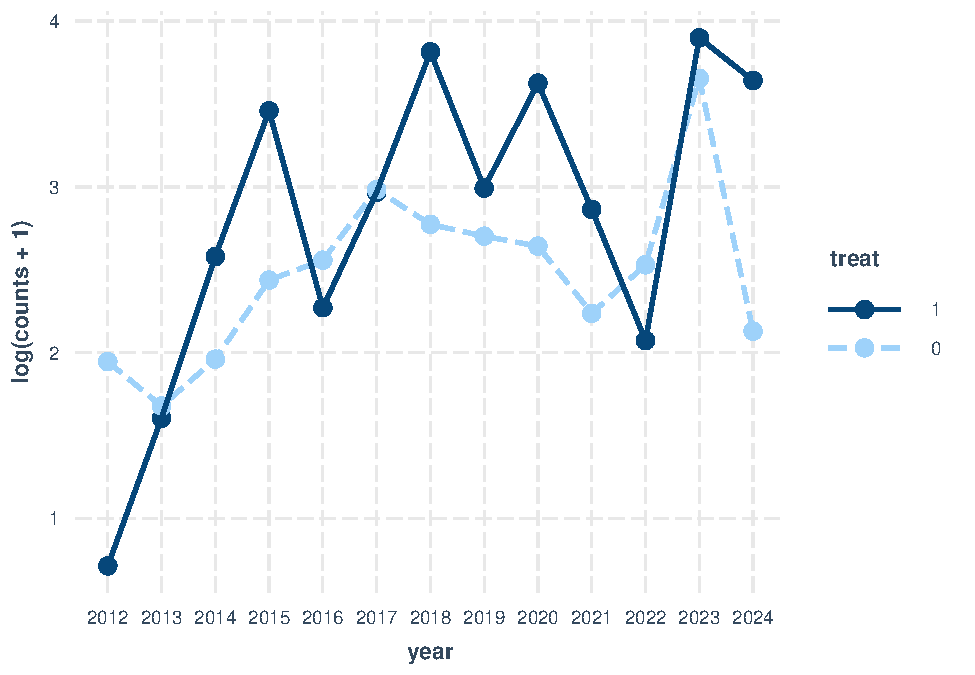
\includegraphics{hw1-lobstrs-eds241_files/figure-latex/unnamed-chunk-46-1.pdf}

\begin{Shaded}
\begin{Highlighting}[]
\NormalTok{plot\_counts\_recent }\OtherTok{\textless{}{-}}\NormalTok{ recent\_counts }\SpecialCharTok{|\textgreater{}} 
    \FunctionTok{group\_by}\NormalTok{(year, mpa) }\SpecialCharTok{|\textgreater{}} 
    \FunctionTok{summarize}\NormalTok{(}\AttributeTok{mean\_counts =} \FunctionTok{mean}\NormalTok{(counts)) }\SpecialCharTok{|\textgreater{}} 
    \FunctionTok{mutate}\NormalTok{(}\AttributeTok{year =} \FunctionTok{as.factor}\NormalTok{(year)) }\SpecialCharTok{|\textgreater{}} 
    \FunctionTok{ggplot}\NormalTok{(}\FunctionTok{aes}\NormalTok{(}\AttributeTok{x =}\NormalTok{ year, }\AttributeTok{y =}\NormalTok{ mean\_counts, }\AttributeTok{color =}\NormalTok{ mpa)) }\SpecialCharTok{+}
    \FunctionTok{geom\_point}\NormalTok{() }\SpecialCharTok{+}
    \FunctionTok{geom\_line}\NormalTok{(}\FunctionTok{aes}\NormalTok{(}\AttributeTok{group =}\NormalTok{ mpa)) }\SpecialCharTok{+}
    \FunctionTok{labs}\NormalTok{(}
        \AttributeTok{title =} \StringTok{"Treatment Effect (MPA) Changes in Lobster Counts from 2012 to 2024"}\NormalTok{,}
        \AttributeTok{x =} \StringTok{"Year"}\NormalTok{,}
        \AttributeTok{y =} \StringTok{"Mean Lobster Counts"}
\NormalTok{    ) }\SpecialCharTok{+}
    \FunctionTok{scale\_color\_manual}\NormalTok{(}\AttributeTok{values =} \FunctionTok{c}\NormalTok{(}\StringTok{"navy"}\NormalTok{, }\StringTok{"lightblue3"}\NormalTok{ ),}
                       \AttributeTok{labels =} \FunctionTok{c}\NormalTok{(}\StringTok{"MPA"}\NormalTok{, }\StringTok{"Non{-}MPA"}\NormalTok{)) }\SpecialCharTok{+}
    \FunctionTok{scale\_linetype\_manual}\NormalTok{(}\AttributeTok{values =} \FunctionTok{c}\NormalTok{(}\StringTok{"solid"}\NormalTok{, }\StringTok{"longdash"}\NormalTok{))}

\FunctionTok{print}\NormalTok{(plot\_counts\_recent)}
\end{Highlighting}
\end{Shaded}

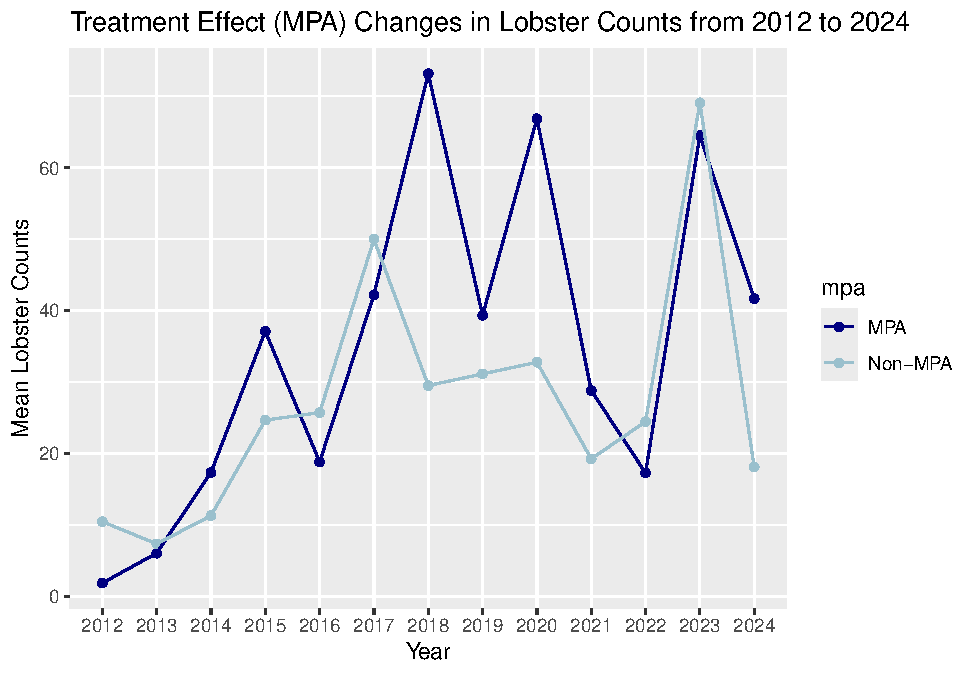
\includegraphics{hw1-lobstrs-eds241_files/figure-latex/unnamed-chunk-47-1.pdf}

\begin{enumerate}
\def\labelenumi{\alph{enumi}.}
\setcounter{enumi}{2}
\tightlist
\item
  Compare and contrast results with the analysis from the 2012-2018 data
  sample (\textasciitilde{} 2 paragraphs)
\end{enumerate}

\begin{Shaded}
\begin{Highlighting}[]
\FunctionTok{export\_summs}\NormalTok{(m1\_ols, m2\_pois, m3\_nb, m1\_ols\_recent, m2\_pois\_recent, m3\_nb\_recent,}
             \AttributeTok{model.names =} \FunctionTok{c}\NormalTok{(}\StringTok{"OLS"}\NormalTok{,}\StringTok{"Poisson"}\NormalTok{, }\StringTok{"NB"}\NormalTok{, }\StringTok{"2024 OLS"}\NormalTok{, }\StringTok{"2024 Poisson"}\NormalTok{, }\StringTok{"2024 NB"}\NormalTok{))}
\end{Highlighting}
\end{Shaded}

 
  \providecommand{\huxb}[2]{\arrayrulecolor[RGB]{#1}\global\arrayrulewidth=#2pt}
  \providecommand{\huxvb}[2]{\color[RGB]{#1}\vrule width #2pt}
  \providecommand{\huxtpad}[1]{\rule{0pt}{#1}}
  \providecommand{\huxbpad}[1]{\rule[-#1]{0pt}{#1}}

\begin{table}[ht]
\begin{centerbox}
\begin{threeparttable}
 \setlength{\tabcolsep}{0pt}
\begin{tabular}{l l l l l l l}


\hhline{>{\huxb{0, 0, 0}{0.8}}->{\huxb{0, 0, 0}{0.8}}->{\huxb{0, 0, 0}{0.8}}->{\huxb{0, 0, 0}{0.8}}->{\huxb{0, 0, 0}{0.8}}->{\huxb{0, 0, 0}{0.8}}->{\huxb{0, 0, 0}{0.8}}-}
\arrayrulecolor{black}

\multicolumn{1}{!{\huxvb{0, 0, 0}{0}}c!{\huxvb{0, 0, 0}{0}}}{\huxtpad{6pt + 1em}\centering \hspace{6pt}  \hspace{6pt}\huxbpad{6pt}} &
\multicolumn{1}{c!{\huxvb{0, 0, 0}{0}}}{\huxtpad{6pt + 1em}\centering \hspace{6pt} OLS \hspace{6pt}\huxbpad{6pt}} &
\multicolumn{1}{c!{\huxvb{0, 0, 0}{0}}}{\huxtpad{6pt + 1em}\centering \hspace{6pt} Poisson \hspace{6pt}\huxbpad{6pt}} &
\multicolumn{1}{c!{\huxvb{0, 0, 0}{0}}}{\huxtpad{6pt + 1em}\centering \hspace{6pt} NB \hspace{6pt}\huxbpad{6pt}} &
\multicolumn{1}{c!{\huxvb{0, 0, 0}{0}}}{\huxtpad{6pt + 1em}\centering \hspace{6pt} 2024 OLS \hspace{6pt}\huxbpad{6pt}} &
\multicolumn{1}{c!{\huxvb{0, 0, 0}{0}}}{\huxtpad{6pt + 1em}\centering \hspace{6pt} 2024 Poisson \hspace{6pt}\huxbpad{6pt}} &
\multicolumn{1}{c!{\huxvb{0, 0, 0}{0}}}{\huxtpad{6pt + 1em}\centering \hspace{6pt} 2024 NB \hspace{6pt}\huxbpad{6pt}} \tabularnewline[-0.5pt]


\hhline{>{\huxb{255, 255, 255}{0.4}}->{\huxb{0, 0, 0}{0.4}}->{\huxb{0, 0, 0}{0.4}}->{\huxb{0, 0, 0}{0.4}}->{\huxb{0, 0, 0}{0.4}}->{\huxb{0, 0, 0}{0.4}}->{\huxb{0, 0, 0}{0.4}}-}
\arrayrulecolor{black}

\multicolumn{1}{!{\huxvb{0, 0, 0}{0}}l!{\huxvb{0, 0, 0}{0}}}{\huxtpad{6pt + 1em}\raggedright \hspace{6pt} (Intercept) \hspace{6pt}\huxbpad{6pt}} &
\multicolumn{1}{r!{\huxvb{0, 0, 0}{0}}}{\huxtpad{6pt + 1em}\raggedleft \hspace{6pt} 22.73 *** \hspace{6pt}\huxbpad{6pt}} &
\multicolumn{1}{r!{\huxvb{0, 0, 0}{0}}}{\huxtpad{6pt + 1em}\raggedleft \hspace{6pt} 3.12 *** \hspace{6pt}\huxbpad{6pt}} &
\multicolumn{1}{r!{\huxvb{0, 0, 0}{0}}}{\huxtpad{6pt + 1em}\raggedleft \hspace{6pt} 3.12 *** \hspace{6pt}\huxbpad{6pt}} &
\multicolumn{1}{r!{\huxvb{0, 0, 0}{0}}}{\huxtpad{6pt + 1em}\raggedleft \hspace{6pt} 27.27 *** \hspace{6pt}\huxbpad{6pt}} &
\multicolumn{1}{r!{\huxvb{0, 0, 0}{0}}}{\huxtpad{6pt + 1em}\raggedleft \hspace{6pt} 3.31 *** \hspace{6pt}\huxbpad{6pt}} &
\multicolumn{1}{r!{\huxvb{0, 0, 0}{0}}}{\huxtpad{6pt + 1em}\raggedleft \hspace{6pt} 3.31 *** \hspace{6pt}\huxbpad{6pt}} \tabularnewline[-0.5pt]


\hhline{}
\arrayrulecolor{black}

\multicolumn{1}{!{\huxvb{0, 0, 0}{0}}l!{\huxvb{0, 0, 0}{0}}}{\huxtpad{6pt + 1em}\raggedright \hspace{6pt}  \hspace{6pt}\huxbpad{6pt}} &
\multicolumn{1}{r!{\huxvb{0, 0, 0}{0}}}{\huxtpad{6pt + 1em}\raggedleft \hspace{6pt} (3.57)\hphantom{0}\hphantom{0}\hphantom{0} \hspace{6pt}\huxbpad{6pt}} &
\multicolumn{1}{r!{\huxvb{0, 0, 0}{0}}}{\huxtpad{6pt + 1em}\raggedleft \hspace{6pt} (0.02)\hphantom{0}\hphantom{0}\hphantom{0} \hspace{6pt}\huxbpad{6pt}} &
\multicolumn{1}{r!{\huxvb{0, 0, 0}{0}}}{\huxtpad{6pt + 1em}\raggedleft \hspace{6pt} (0.12)\hphantom{0}\hphantom{0}\hphantom{0} \hspace{6pt}\huxbpad{6pt}} &
\multicolumn{1}{r!{\huxvb{0, 0, 0}{0}}}{\huxtpad{6pt + 1em}\raggedleft \hspace{6pt} (2.69)\hphantom{0}\hphantom{0}\hphantom{0} \hspace{6pt}\huxbpad{6pt}} &
\multicolumn{1}{r!{\huxvb{0, 0, 0}{0}}}{\huxtpad{6pt + 1em}\raggedleft \hspace{6pt} (0.01)\hphantom{0}\hphantom{0}\hphantom{0} \hspace{6pt}\huxbpad{6pt}} &
\multicolumn{1}{r!{\huxvb{0, 0, 0}{0}}}{\huxtpad{6pt + 1em}\raggedleft \hspace{6pt} (0.08)\hphantom{0}\hphantom{0}\hphantom{0} \hspace{6pt}\huxbpad{6pt}} \tabularnewline[-0.5pt]


\hhline{}
\arrayrulecolor{black}

\multicolumn{1}{!{\huxvb{0, 0, 0}{0}}l!{\huxvb{0, 0, 0}{0}}}{\huxtpad{6pt + 1em}\raggedright \hspace{6pt} treat \hspace{6pt}\huxbpad{6pt}} &
\multicolumn{1}{r!{\huxvb{0, 0, 0}{0}}}{\huxtpad{6pt + 1em}\raggedleft \hspace{6pt} 5.36\hphantom{0}\hphantom{0}\hphantom{0}\hphantom{0} \hspace{6pt}\huxbpad{6pt}} &
\multicolumn{1}{r!{\huxvb{0, 0, 0}{0}}}{\huxtpad{6pt + 1em}\raggedleft \hspace{6pt} 0.21 *** \hspace{6pt}\huxbpad{6pt}} &
\multicolumn{1}{r!{\huxvb{0, 0, 0}{0}}}{\huxtpad{6pt + 1em}\raggedleft \hspace{6pt} 0.21\hphantom{0}\hphantom{0}\hphantom{0}\hphantom{0} \hspace{6pt}\huxbpad{6pt}} &
\multicolumn{1}{r!{\huxvb{0, 0, 0}{0}}}{\huxtpad{6pt + 1em}\raggedleft \hspace{6pt} 7.72 *\hphantom{0}\hphantom{0} \hspace{6pt}\huxbpad{6pt}} &
\multicolumn{1}{r!{\huxvb{0, 0, 0}{0}}}{\huxtpad{6pt + 1em}\raggedleft \hspace{6pt} 0.25 *** \hspace{6pt}\huxbpad{6pt}} &
\multicolumn{1}{r!{\huxvb{0, 0, 0}{0}}}{\huxtpad{6pt + 1em}\raggedleft \hspace{6pt} 0.25 *\hphantom{0}\hphantom{0} \hspace{6pt}\huxbpad{6pt}} \tabularnewline[-0.5pt]


\hhline{}
\arrayrulecolor{black}

\multicolumn{1}{!{\huxvb{0, 0, 0}{0}}l!{\huxvb{0, 0, 0}{0}}}{\huxtpad{6pt + 1em}\raggedright \hspace{6pt}  \hspace{6pt}\huxbpad{6pt}} &
\multicolumn{1}{r!{\huxvb{0, 0, 0}{0}}}{\huxtpad{6pt + 1em}\raggedleft \hspace{6pt} (5.20)\hphantom{0}\hphantom{0}\hphantom{0} \hspace{6pt}\huxbpad{6pt}} &
\multicolumn{1}{r!{\huxvb{0, 0, 0}{0}}}{\huxtpad{6pt + 1em}\raggedleft \hspace{6pt} (0.03)\hphantom{0}\hphantom{0}\hphantom{0} \hspace{6pt}\huxbpad{6pt}} &
\multicolumn{1}{r!{\huxvb{0, 0, 0}{0}}}{\huxtpad{6pt + 1em}\raggedleft \hspace{6pt} (0.17)\hphantom{0}\hphantom{0}\hphantom{0} \hspace{6pt}\huxbpad{6pt}} &
\multicolumn{1}{r!{\huxvb{0, 0, 0}{0}}}{\huxtpad{6pt + 1em}\raggedleft \hspace{6pt} (3.91)\hphantom{0}\hphantom{0}\hphantom{0} \hspace{6pt}\huxbpad{6pt}} &
\multicolumn{1}{r!{\huxvb{0, 0, 0}{0}}}{\huxtpad{6pt + 1em}\raggedleft \hspace{6pt} (0.02)\hphantom{0}\hphantom{0}\hphantom{0} \hspace{6pt}\huxbpad{6pt}} &
\multicolumn{1}{r!{\huxvb{0, 0, 0}{0}}}{\huxtpad{6pt + 1em}\raggedleft \hspace{6pt} (0.12)\hphantom{0}\hphantom{0}\hphantom{0} \hspace{6pt}\huxbpad{6pt}} \tabularnewline[-0.5pt]


\hhline{>{\huxb{255, 255, 255}{0.4}}->{\huxb{0, 0, 0}{0.4}}->{\huxb{0, 0, 0}{0.4}}->{\huxb{0, 0, 0}{0.4}}->{\huxb{0, 0, 0}{0.4}}->{\huxb{0, 0, 0}{0.4}}->{\huxb{0, 0, 0}{0.4}}-}
\arrayrulecolor{black}

\multicolumn{1}{!{\huxvb{0, 0, 0}{0}}l!{\huxvb{0, 0, 0}{0}}}{\huxtpad{6pt + 1em}\raggedright \hspace{6pt} N \hspace{6pt}\huxbpad{6pt}} &
\multicolumn{1}{r!{\huxvb{0, 0, 0}{0}}}{\huxtpad{6pt + 1em}\raggedleft \hspace{6pt} 252\hphantom{0}\hphantom{0}\hphantom{0}\hphantom{0}\hphantom{0}\hphantom{0}\hphantom{0} \hspace{6pt}\huxbpad{6pt}} &
\multicolumn{1}{r!{\huxvb{0, 0, 0}{0}}}{\huxtpad{6pt + 1em}\raggedleft \hspace{6pt} 252\hphantom{0}\hphantom{0}\hphantom{0}\hphantom{0}\hphantom{0}\hphantom{0}\hphantom{0} \hspace{6pt}\huxbpad{6pt}} &
\multicolumn{1}{r!{\huxvb{0, 0, 0}{0}}}{\huxtpad{6pt + 1em}\raggedleft \hspace{6pt} 252\hphantom{0}\hphantom{0}\hphantom{0}\hphantom{0}\hphantom{0}\hphantom{0}\hphantom{0} \hspace{6pt}\huxbpad{6pt}} &
\multicolumn{1}{r!{\huxvb{0, 0, 0}{0}}}{\huxtpad{6pt + 1em}\raggedleft \hspace{6pt} 466\hphantom{0}\hphantom{0}\hphantom{0}\hphantom{0}\hphantom{0}\hphantom{0}\hphantom{0} \hspace{6pt}\huxbpad{6pt}} &
\multicolumn{1}{r!{\huxvb{0, 0, 0}{0}}}{\huxtpad{6pt + 1em}\raggedleft \hspace{6pt} 466\hphantom{0}\hphantom{0}\hphantom{0}\hphantom{0}\hphantom{0}\hphantom{0}\hphantom{0} \hspace{6pt}\huxbpad{6pt}} &
\multicolumn{1}{r!{\huxvb{0, 0, 0}{0}}}{\huxtpad{6pt + 1em}\raggedleft \hspace{6pt} 466\hphantom{0}\hphantom{0}\hphantom{0}\hphantom{0}\hphantom{0}\hphantom{0}\hphantom{0} \hspace{6pt}\huxbpad{6pt}} \tabularnewline[-0.5pt]


\hhline{}
\arrayrulecolor{black}

\multicolumn{1}{!{\huxvb{0, 0, 0}{0}}l!{\huxvb{0, 0, 0}{0}}}{\huxtpad{6pt + 1em}\raggedright \hspace{6pt} R2 \hspace{6pt}\huxbpad{6pt}} &
\multicolumn{1}{r!{\huxvb{0, 0, 0}{0}}}{\huxtpad{6pt + 1em}\raggedleft \hspace{6pt} 0.00\hphantom{0}\hphantom{0}\hphantom{0}\hphantom{0} \hspace{6pt}\huxbpad{6pt}} &
\multicolumn{1}{r!{\huxvb{0, 0, 0}{0}}}{\huxtpad{6pt + 1em}\raggedleft \hspace{6pt} \hphantom{0}\hphantom{0}\hphantom{0}\hphantom{0}\hphantom{0}\hphantom{0}\hphantom{0} \hspace{6pt}\huxbpad{6pt}} &
\multicolumn{1}{r!{\huxvb{0, 0, 0}{0}}}{\huxtpad{6pt + 1em}\raggedleft \hspace{6pt} \hphantom{0}\hphantom{0}\hphantom{0}\hphantom{0}\hphantom{0}\hphantom{0}\hphantom{0} \hspace{6pt}\huxbpad{6pt}} &
\multicolumn{1}{r!{\huxvb{0, 0, 0}{0}}}{\huxtpad{6pt + 1em}\raggedleft \hspace{6pt} 0.01\hphantom{0}\hphantom{0}\hphantom{0}\hphantom{0} \hspace{6pt}\huxbpad{6pt}} &
\multicolumn{1}{r!{\huxvb{0, 0, 0}{0}}}{\huxtpad{6pt + 1em}\raggedleft \hspace{6pt} \hphantom{0}\hphantom{0}\hphantom{0}\hphantom{0}\hphantom{0}\hphantom{0}\hphantom{0} \hspace{6pt}\huxbpad{6pt}} &
\multicolumn{1}{r!{\huxvb{0, 0, 0}{0}}}{\huxtpad{6pt + 1em}\raggedleft \hspace{6pt} \hphantom{0}\hphantom{0}\hphantom{0}\hphantom{0}\hphantom{0}\hphantom{0}\hphantom{0} \hspace{6pt}\huxbpad{6pt}} \tabularnewline[-0.5pt]


\hhline{}
\arrayrulecolor{black}

\multicolumn{1}{!{\huxvb{0, 0, 0}{0}}l!{\huxvb{0, 0, 0}{0}}}{\huxtpad{6pt + 1em}\raggedright \hspace{6pt} AIC \hspace{6pt}\huxbpad{6pt}} &
\multicolumn{1}{r!{\huxvb{0, 0, 0}{0}}}{\huxtpad{6pt + 1em}\raggedleft \hspace{6pt} 2593.35\hphantom{0}\hphantom{0}\hphantom{0}\hphantom{0} \hspace{6pt}\huxbpad{6pt}} &
\multicolumn{1}{r!{\huxvb{0, 0, 0}{0}}}{\huxtpad{6pt + 1em}\raggedleft \hspace{6pt} 11365.62\hphantom{0}\hphantom{0}\hphantom{0}\hphantom{0} \hspace{6pt}\huxbpad{6pt}} &
\multicolumn{1}{r!{\huxvb{0, 0, 0}{0}}}{\huxtpad{6pt + 1em}\raggedleft \hspace{6pt} 2088.53\hphantom{0}\hphantom{0}\hphantom{0}\hphantom{0} \hspace{6pt}\huxbpad{6pt}} &
\multicolumn{1}{r!{\huxvb{0, 0, 0}{0}}}{\huxtpad{6pt + 1em}\raggedleft \hspace{6pt} 4813.06\hphantom{0}\hphantom{0}\hphantom{0}\hphantom{0} \hspace{6pt}\huxbpad{6pt}} &
\multicolumn{1}{r!{\huxvb{0, 0, 0}{0}}}{\huxtpad{6pt + 1em}\raggedleft \hspace{6pt} 21530.09\hphantom{0}\hphantom{0}\hphantom{0}\hphantom{0} \hspace{6pt}\huxbpad{6pt}} &
\multicolumn{1}{r!{\huxvb{0, 0, 0}{0}}}{\huxtpad{6pt + 1em}\raggedleft \hspace{6pt} 4058.04\hphantom{0}\hphantom{0}\hphantom{0}\hphantom{0} \hspace{6pt}\huxbpad{6pt}} \tabularnewline[-0.5pt]


\hhline{}
\arrayrulecolor{black}

\multicolumn{1}{!{\huxvb{0, 0, 0}{0}}l!{\huxvb{0, 0, 0}{0}}}{\huxtpad{6pt + 1em}\raggedright \hspace{6pt} BIC \hspace{6pt}\huxbpad{6pt}} &
\multicolumn{1}{r!{\huxvb{0, 0, 0}{0}}}{\huxtpad{6pt + 1em}\raggedleft \hspace{6pt} 2603.94\hphantom{0}\hphantom{0}\hphantom{0}\hphantom{0} \hspace{6pt}\huxbpad{6pt}} &
\multicolumn{1}{r!{\huxvb{0, 0, 0}{0}}}{\huxtpad{6pt + 1em}\raggedleft \hspace{6pt} 11372.68\hphantom{0}\hphantom{0}\hphantom{0}\hphantom{0} \hspace{6pt}\huxbpad{6pt}} &
\multicolumn{1}{r!{\huxvb{0, 0, 0}{0}}}{\huxtpad{6pt + 1em}\raggedleft \hspace{6pt} 2099.12\hphantom{0}\hphantom{0}\hphantom{0}\hphantom{0} \hspace{6pt}\huxbpad{6pt}} &
\multicolumn{1}{r!{\huxvb{0, 0, 0}{0}}}{\huxtpad{6pt + 1em}\raggedleft \hspace{6pt} 4825.50\hphantom{0}\hphantom{0}\hphantom{0}\hphantom{0} \hspace{6pt}\huxbpad{6pt}} &
\multicolumn{1}{r!{\huxvb{0, 0, 0}{0}}}{\huxtpad{6pt + 1em}\raggedleft \hspace{6pt} 21538.38\hphantom{0}\hphantom{0}\hphantom{0}\hphantom{0} \hspace{6pt}\huxbpad{6pt}} &
\multicolumn{1}{r!{\huxvb{0, 0, 0}{0}}}{\huxtpad{6pt + 1em}\raggedleft \hspace{6pt} 4070.48\hphantom{0}\hphantom{0}\hphantom{0}\hphantom{0} \hspace{6pt}\huxbpad{6pt}} \tabularnewline[-0.5pt]


\hhline{}
\arrayrulecolor{black}

\multicolumn{1}{!{\huxvb{0, 0, 0}{0}}l!{\huxvb{0, 0, 0}{0}}}{\huxtpad{6pt + 1em}\raggedright \hspace{6pt} Pseudo R2 \hspace{6pt}\huxbpad{6pt}} &
\multicolumn{1}{r!{\huxvb{0, 0, 0}{0}}}{\huxtpad{6pt + 1em}\raggedleft \hspace{6pt} \hphantom{0}\hphantom{0}\hphantom{0}\hphantom{0}\hphantom{0}\hphantom{0}\hphantom{0} \hspace{6pt}\huxbpad{6pt}} &
\multicolumn{1}{r!{\huxvb{0, 0, 0}{0}}}{\huxtpad{6pt + 1em}\raggedleft \hspace{6pt} 0.25\hphantom{0}\hphantom{0}\hphantom{0}\hphantom{0} \hspace{6pt}\huxbpad{6pt}} &
\multicolumn{1}{r!{\huxvb{0, 0, 0}{0}}}{\huxtpad{6pt + 1em}\raggedleft \hspace{6pt} 0.01\hphantom{0}\hphantom{0}\hphantom{0}\hphantom{0} \hspace{6pt}\huxbpad{6pt}} &
\multicolumn{1}{r!{\huxvb{0, 0, 0}{0}}}{\huxtpad{6pt + 1em}\raggedleft \hspace{6pt} \hphantom{0}\hphantom{0}\hphantom{0}\hphantom{0}\hphantom{0}\hphantom{0}\hphantom{0} \hspace{6pt}\huxbpad{6pt}} &
\multicolumn{1}{r!{\huxvb{0, 0, 0}{0}}}{\huxtpad{6pt + 1em}\raggedleft \hspace{6pt} 0.38\hphantom{0}\hphantom{0}\hphantom{0}\hphantom{0} \hspace{6pt}\huxbpad{6pt}} &
\multicolumn{1}{r!{\huxvb{0, 0, 0}{0}}}{\huxtpad{6pt + 1em}\raggedleft \hspace{6pt} 0.01\hphantom{0}\hphantom{0}\hphantom{0}\hphantom{0} \hspace{6pt}\huxbpad{6pt}} \tabularnewline[-0.5pt]


\hhline{>{\huxb{0, 0, 0}{0.8}}->{\huxb{0, 0, 0}{0.8}}->{\huxb{0, 0, 0}{0.8}}->{\huxb{0, 0, 0}{0.8}}->{\huxb{0, 0, 0}{0.8}}->{\huxb{0, 0, 0}{0.8}}->{\huxb{0, 0, 0}{0.8}}-}
\arrayrulecolor{black}

\multicolumn{7}{!{\huxvb{0, 0, 0}{0}}l!{\huxvb{0, 0, 0}{0}}}{\huxtpad{6pt + 1em}\raggedright \hspace{6pt}  *** p $<$ 0.001;  ** p $<$ 0.01;  * p $<$ 0.05. \hspace{6pt}\huxbpad{6pt}} \tabularnewline[-0.5pt]


\hhline{}
\arrayrulecolor{black}
\end{tabular}
\end{threeparttable}\par\end{centerbox}

\end{table}
 

The results of the original OLS analysis versus this new one differs by
2.36. This result isn't surprising because we see a significant spike in
2018 - 2020 for MPA sites over non-MPA sites. This spike isn't seen in
the original OLS analysis because it ends at 2018. The results of the
original Poisson analysis versus this one differs by 5.03\%. Once again,
it makes sense that the recent poisson model has a bigger treatment
effect because of the spike that is unaccounted for in the first model.
Like the previous model, this recent Negative Binomial model has the
same treatment effect as the Poisson model.

When looking at the plots, we can see that after the spike from
2018-2020, the MPA site actually dips lower in counts than the non-MPA
sites. There is also a significant spike in both MPA and non-MPA sites
in 2023. My theory is that the spillover effect that we are seeing in
the original data is continuing even more here. As the spillover builds
up, it makes the non-MPA sites follow the trends of the MPA sites.

\begin{center}\rule{0.5\linewidth}{0.5pt}\end{center}

\includegraphics{figures/spiny1.png}

\end{document}
